\documentclass[11pt]{beamer}
\usetheme[progressbar=head,block=fill]{metropolis}
\setbeamercolor{background canvas}{bg=white}

\usepackage[backend=biber,style=authoryear, defernumbers=true]{biblatex}
\addbibresource{refs.bib}
\usepackage{cancel}
\usepackage{caption}
\captionsetup[figure]{labelformat=empty}
\usepackage{subcaption}
\usepackage{dsfont}
\usepackage[bold]{hhtensor}
\usepackage{braket}
\usepackage{mathtools}
\usepackage{booktabs}
\usepackage{cleveref}
\usepackage{listings}
\lstset{basicstyle=\tiny}
\usepackage[bold]{hhtensor}
\usepackage{pgfpages}
\usepackage{tikz,pgfplots}
\pgfplotsset{compat=newest}
\usetikzlibrary{patterns}
\usepackage{tkz-euclide}    
\usepackage[ruled]{algorithm2e}
\usepackage[append]{beamersubframe}
\usepackage{multirow}




\newcommand{\EE}{\mathbb{E}}
\newcommand{\E}{\mathbb{E}}
\newcommand{\PP}{\mathbb{P}}
\newcommand{\RR}{\mathbb{R}}
\newcommand{\cE}{\mathcal{E}}
\newcommand{\cL}{\mathcal{L}}
\newcommand{\cN}{\mathcal{N}}
\newcommand{\cO}{\mathcal{O}}
\newcommand{\cQ}{\mathcal{Q}}
\newcommand{\cS}{\mathcal{S}}
\newcommand{\dd}{\vec{d}}
\newcommand{\mI}{\matr{I}}
\newcommand{\simiid}{\overset{\text{i.i.d.}}{\sim}}
\DeclareMathOperator*{\argmin}{arg\,min}
\def\A{\matr{A}}
\newcommand{\B}{\matr{B}}
\newcommand{\X}{\matr{X}}
\newcommand{\Z}{\matr{Z}}
\def\Xbb{\overline{\X}}
\def\Xb{{\bar{\X}}}
\newcommand{\Sigmab}{\matr{\Sigma}}
\newcommand{\I}{\matr{I}}
\renewcommand{\x}{\vec{x}}
\def\v{\vec{v}}
\def\xbb{\bar{\mathbf x}}
\newcommand{\y}{\vec{y}}
\newcommand{\yb}{\vec{y}}
\def\ybb{\overline{\y}}
\newcommand{\w}{{\vec{w}}}
\newcommand{\MSE}[1] {{\mathrm{MSE}\big[#1\big]}}
\newcommand{\xib}{\vec{\xi}}
\newcommand{\Nc}{\mathcal{N}}
\newcommand{\zero}{\vec{0}}
\DeclareMathOperator*{\tr}{tr}
\newcommand{\ee}{\vec{e}}
\def\wbh{\widehat{\mathbf w}}
\newcommand{\Bc}{\mathcal{B}}
\newcommand{\Vc}{\mathcal{V}}
\newcommand{\Ic}{\mathcal{I}}
\newcommand{\Jc}{\mathcal{J}}
\DeclareMathOperator{\Det}{Det}
\DeclareMathOperator{\pdet}{pdet}
\DeclareMathOperator{\Poisson}{Poisson}
\DeclareMathOperator{\rank}{rank}
\DeclareMathOperator{\Var}{Var}
\newcommand{\dxy}{\mathrm{D}}
\newcommand{\of}[2]{{#1{\!\ofsub{#2}}}}
\newcommand{\ofsub}[1]{\mbox{\small \raisebox{0.0pt}{$(#1)$}}}
\newcommand{\Red}[1]{\textcolor{red}{#1}}
\newcommand{\Green}[1]{\textcolor{green}{#1}}
\newcommand{\Blue}[1]{\textcolor{blue}{#1}}
\newcommand{\dx}{\dxy_{\!\cal X}}
\newcommand{\R}{\mathbb{R}}
\newcommand{\dxk}{\dxy_{\!\cal X}^k}
\newcommand{\vs}[1]{{\mathrm{VS}_{\!D}^{#1}}}
\def\vsd{{\mathrm{VS}_{\!D}^d}}
\def\vsk{{\mathrm{VS}_{\!D}^k}}
\def\vskx{{\mathrm{VS}_{\!\dx}^k}}
\def\vsdx{{\mathrm{VS}_{\!\dx}^d}}
\def\Xt{\widetilde{X}}
\def\xbt{\widetilde{\x}}
\def\yt{\widetilde{y}}
\def\ytb{\tilde{\mathbf{y}}}
\def\ybt{\widetilde{\mathbf y}}
\newcommand{\defeq}{\stackrel{\textit{\tiny{def}}}{=}}
\newcommand{\Wc}{\mathcal{W}}
\newcommand{\Fc}{\mathcal{F}}
\def\opt{{\textsc{OPT}_k}}
\def\xmark{\Red{\large\sffamily x}}
\def\cmark{\Green{\checkmark}}
\renewcommand{\P}{\matr{P}}
\def\S{\matr{S}}
\def\b{\vec{b}}
\definecolor{reddishyellow}{cmyk}{0,0.22,1.0,0.0}
\definecolor{brightyellow}{cmyk}{0,0,0.7,0.0}
\definecolor{lightyellow}{cmyk}{0,0,0.3,0.0}
\definecolor{lighteryellow}{cmyk}{0,0,0.1,0.0}
\definecolor{lightestyellow}{cmyk}{0,0,0.05,0.0}
\newcommand{\white}[1]{{\textcolor{white}{#1}}}

\newtheorem{proposition}{Proposition}
\newtheorem{assumption}{Assumption}
\newtheorem{remark}{Remark}
\newtheorem{conjecture}{Conjecture}



\title{Randomized tools for inference and analysis}
\subtitle{Thesis Talk, Mahoney Group Meeting}
\author{Feynman Liang}
\institute{UC Berkeley}
\date{\today}


\AtBeginSection[]
{
    \begin{frame}
        \frametitle{Table of Contents}
        \setcounter{tocdepth}{1}
        \tableofcontents[currentsection]
    \end{frame}
}


\begin{document}

\begin{frame}
\titlepage
\end{frame}

% \begin{frame}{Collaborators}
    \begin{columns}[c]
    \begin{column}{0.24\textwidth}
    \begin{figure}
        \centering
        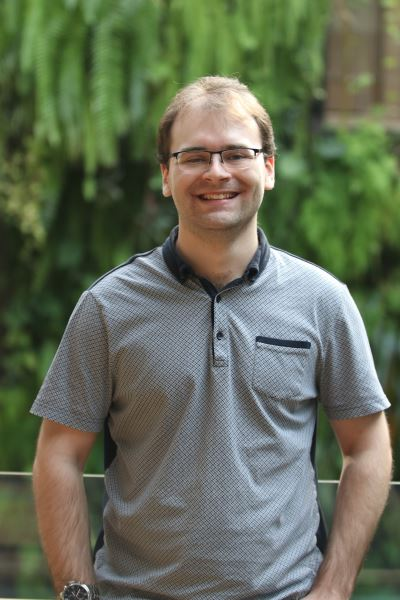
\includegraphics[width=\textwidth,clip,trim={0 7cm 0 0}]{Figures/intro/liam.jpg}
        \caption{\tiny Liam Hodgkinson,\\U Melbourne}
    \end{figure}
    \end{column}
    \begin{column}{0.24\textwidth}
    \begin{figure}
        \centering
        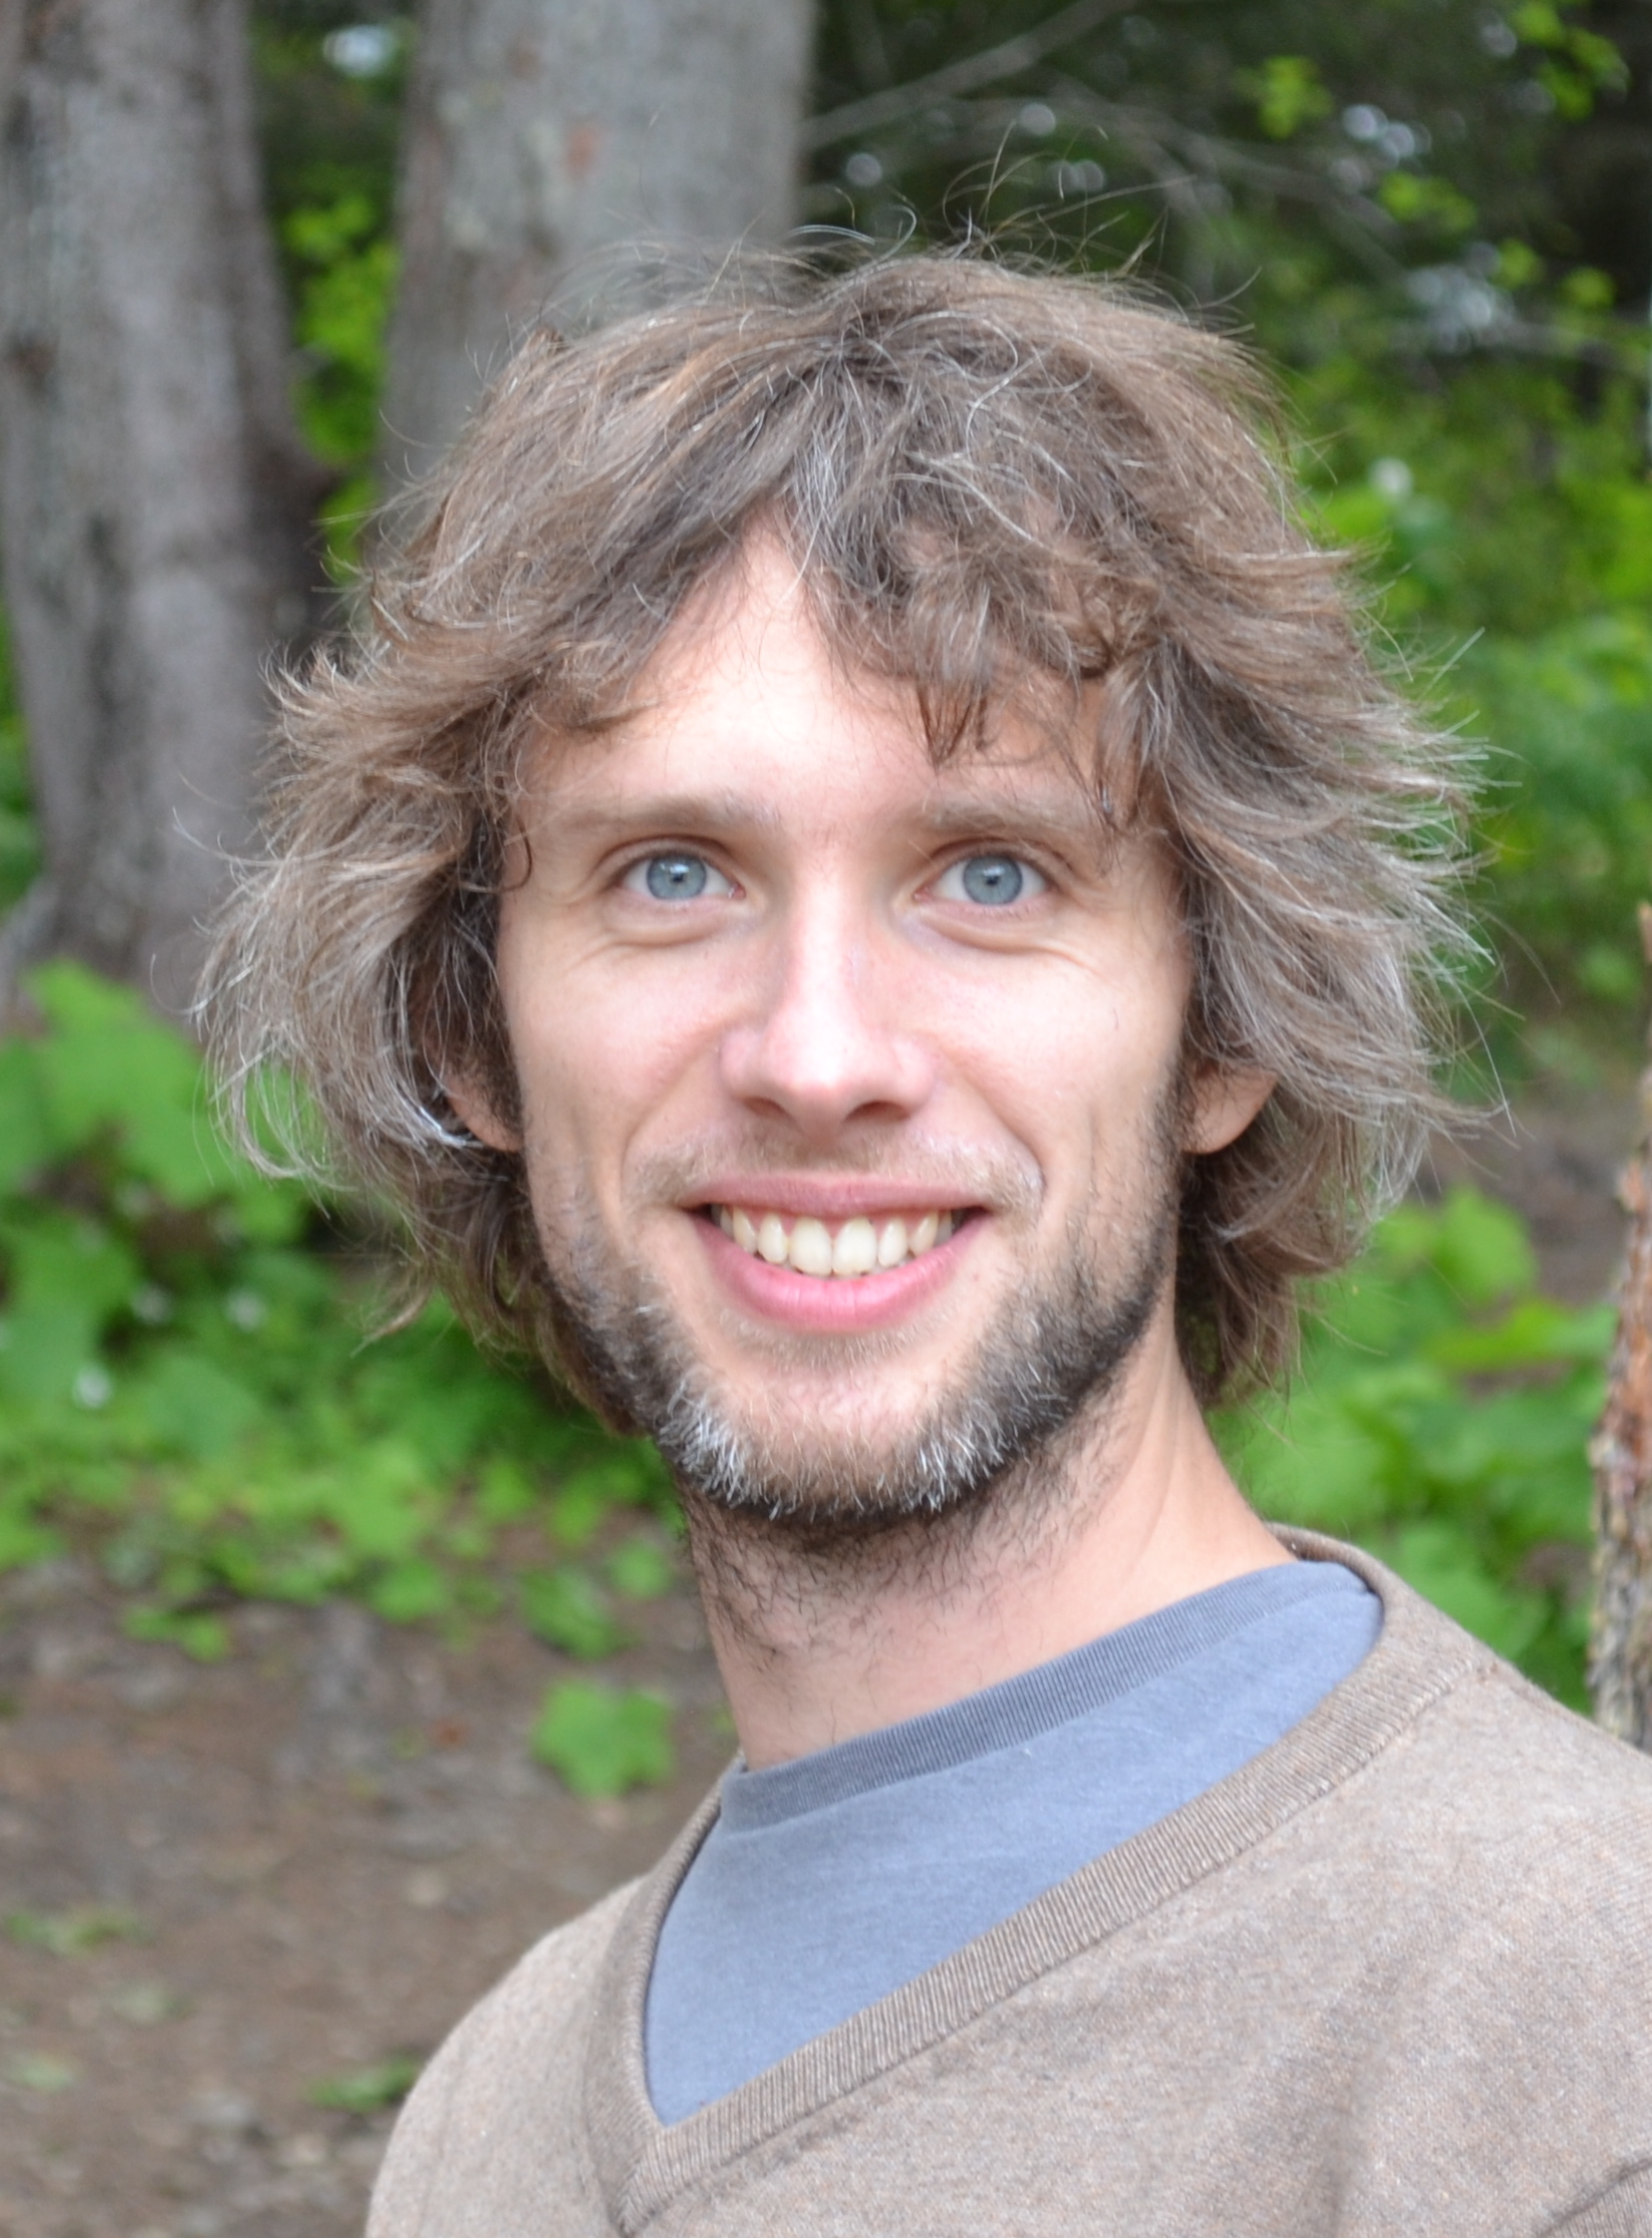
\includegraphics[width=\textwidth,clip,trim={0 3cm 0 2cm}]{Figures/intro/michal.jpg}
        \caption{\tiny Michał Dereziński,\\ U Michigan}
    \end{figure}
    \end{column}
    \begin{column}{0.24\textwidth}
    \begin{figure}
        \centering
        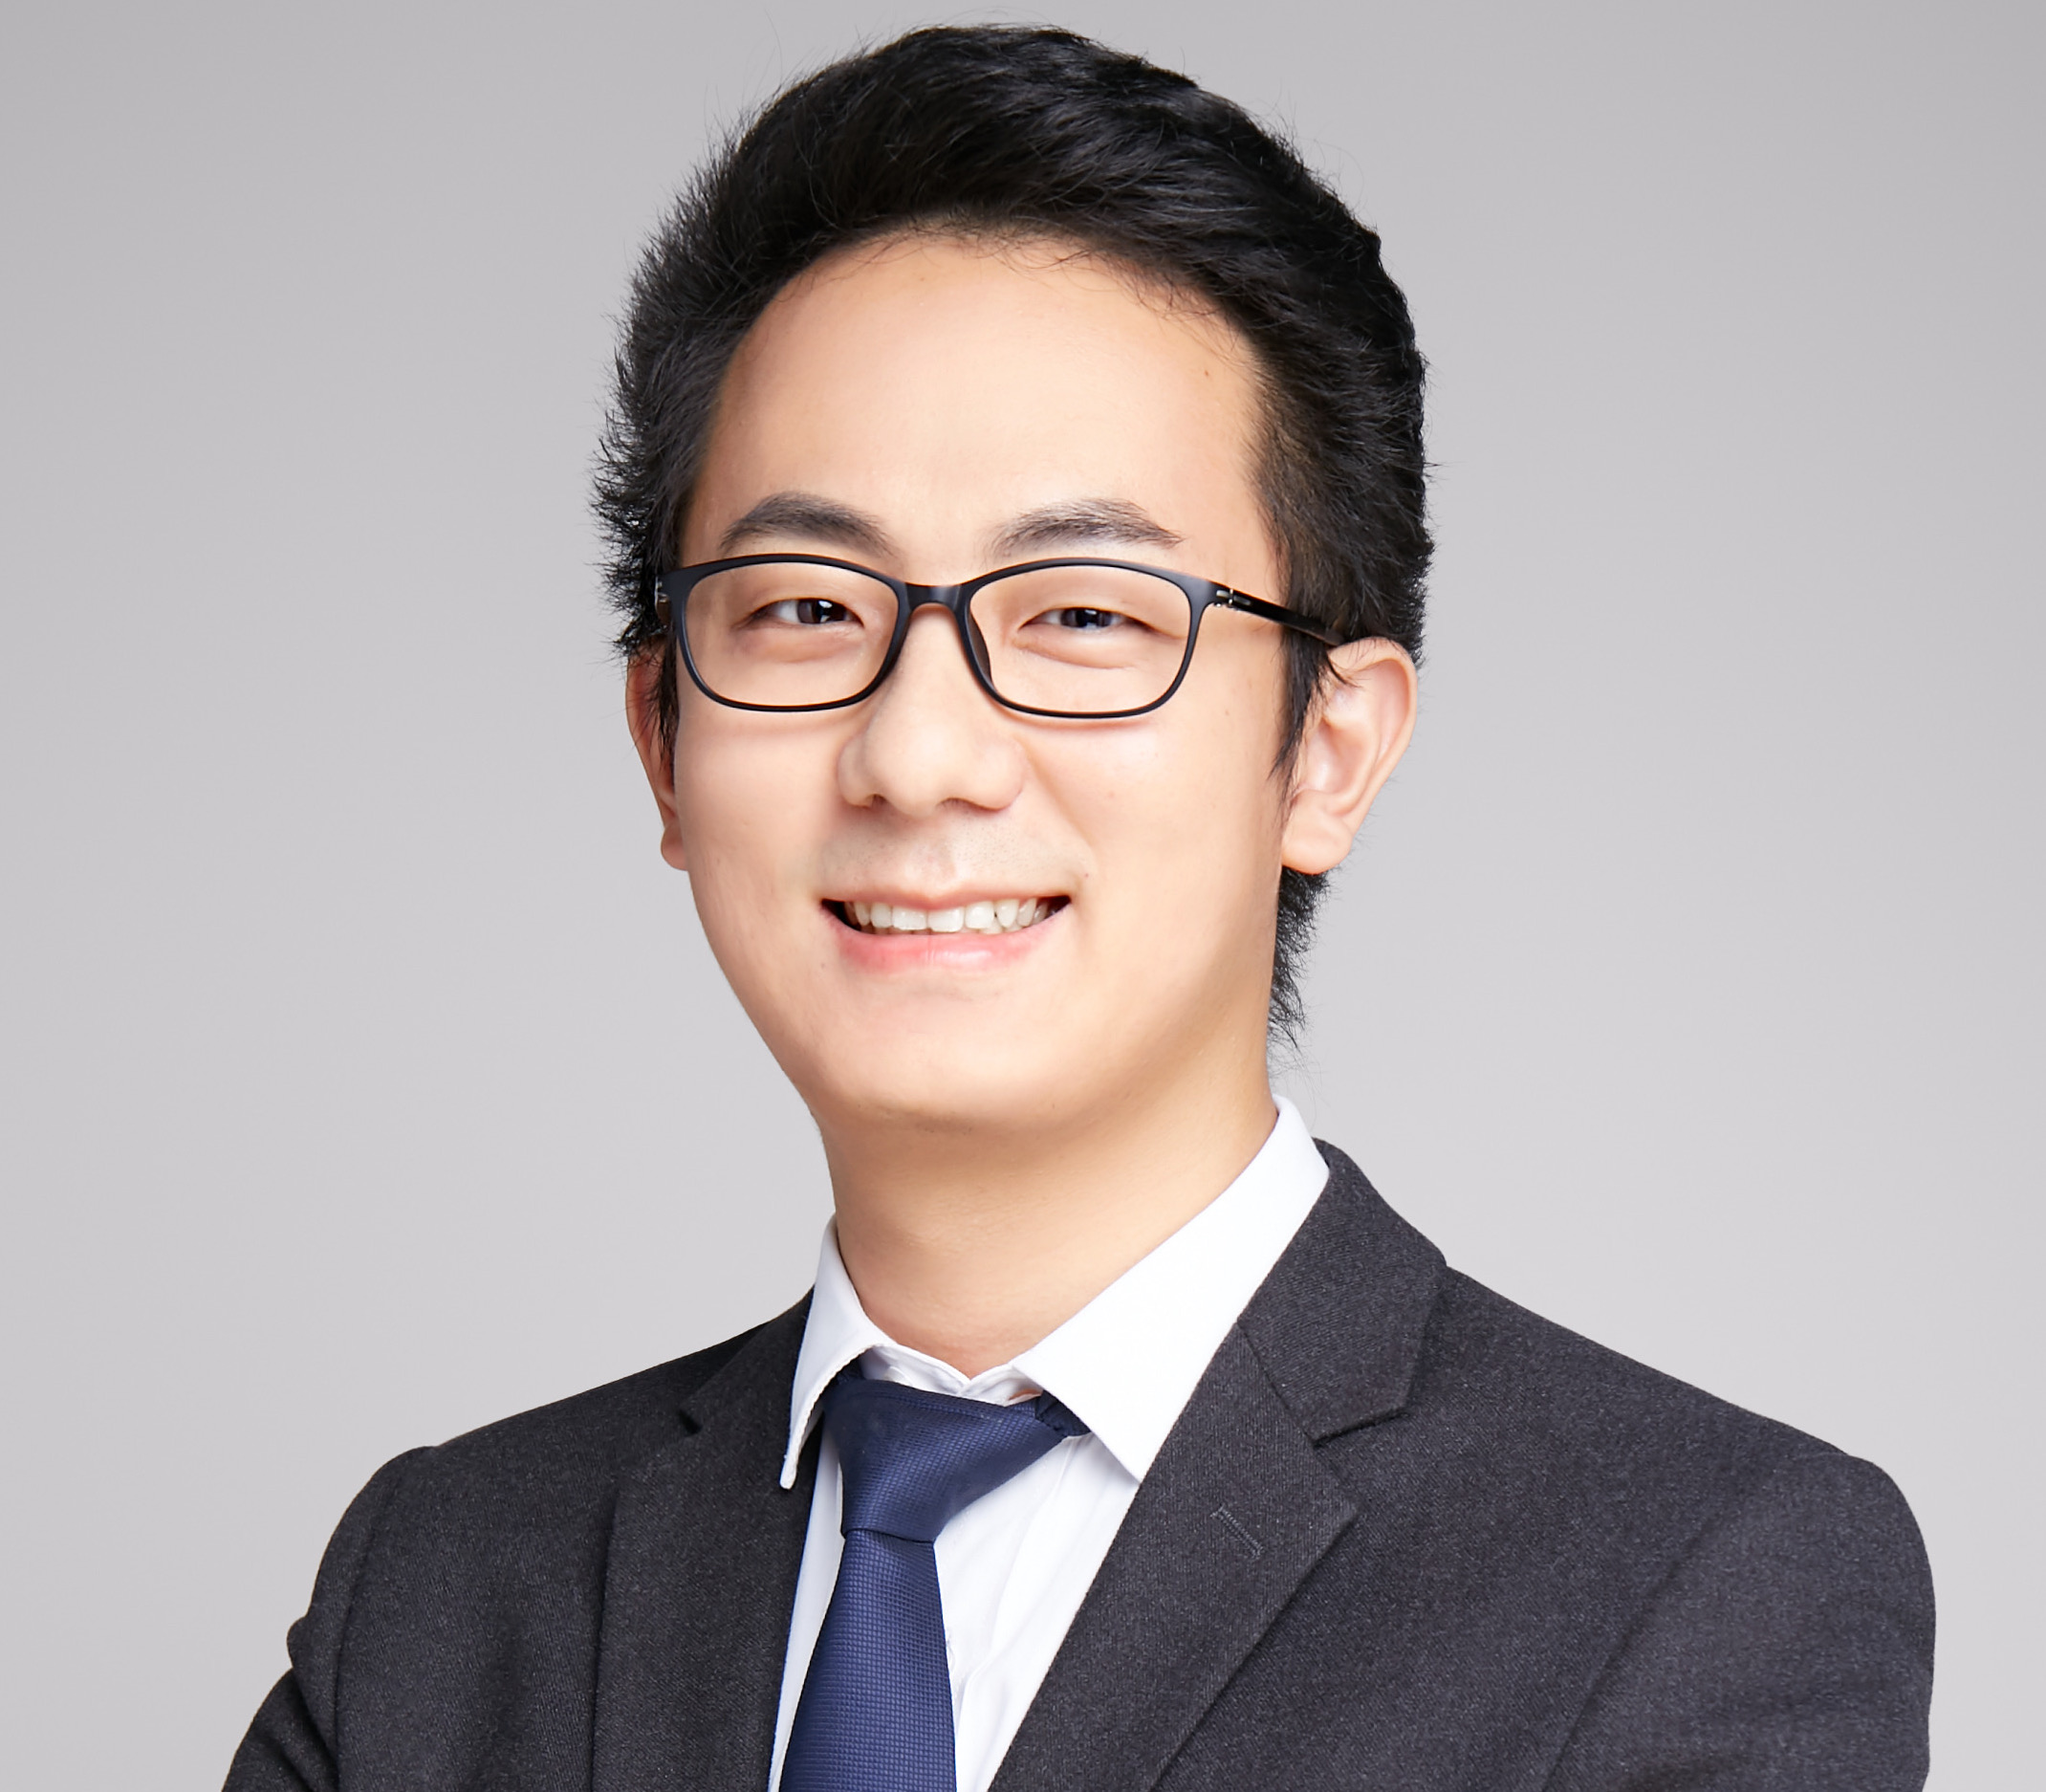
\includegraphics[width=\textwidth,clip,trim={8cm 0 3cm 0}]{Figures/intro/zhenyu.jpeg}
        \caption{\tiny Zhenyu Liao,\\ HUST}
    \end{figure}
    \end{column}
    \begin{column}{0.24\textwidth}
    \begin{figure}
        \centering
        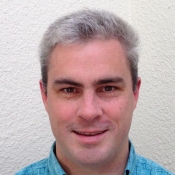
\includegraphics[width=\textwidth]{Figures/intro/mmahoney.png}
        \caption{\tiny Michael Mahoney,\\ UCB/ICSI/LBNL}
    \end{figure}
    \end{column}
    \end{columns}
\end{frame}

\begin{frame}{Committee}
    \begin{columns}[c]
    \begin{column}{0.23\textwidth}
    \begin{figure}
        \centering
        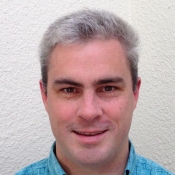
\includegraphics[width=\textwidth]{Figures/intro/mmahoney.png}
        \caption{\tiny Michael Mahoney,\\ Co-Chair}
    \end{figure}
    \end{column}
    \begin{column}{0.23\textwidth}
    \begin{figure}
        \centering
        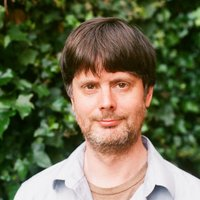
\includegraphics[width=\textwidth,clip,trim={0 0cm 0 0}]{Figures/intro/alan.jpg}
        \caption{\tiny Alan Hammond,\\ Co-Chair}
    \end{figure}
    \end{column}
    \begin{column}{0.23\textwidth}
    \begin{figure}
        \centering
        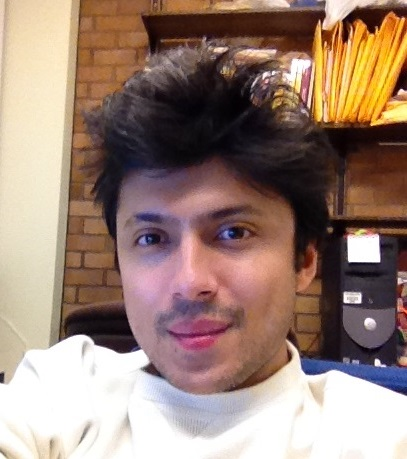
\includegraphics[width=\textwidth,clip,trim={0 1cm 0 0cm}]{Figures/intro/shirsendu.jpg}
        \caption{\tiny Shirsendu Ganguly}
    \end{figure}
    \end{column}
    \begin{column}{0.23\textwidth}
    \begin{figure}
        \centering
        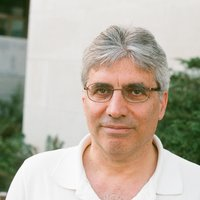
\includegraphics[width=\textwidth,clip,trim={0cm 0 0cm 0}]{Figures/intro/fraydoun.jpg}
        \caption{\tiny Fraydoun Rezakhanlou,\\ ASR}
    \end{figure}
    \end{column}
    \end{columns}
\end{frame}

\begin{frame}{Works Covered}
    
    Probabilistic Programming
    
    {\tiny
    \begin{itemize}
        \item \fullcite{liang2022fat}
        \item \fullcite{gga}
        \item \fullcite{liang2021accelerating}
    \end{itemize}
    }
    
    Theoretical Statistics
    
    {\tiny
    \begin{itemize}
        \item \fullcite{bayesian-experimental-design}
        \item \fullcite{surrogate-design}
        \item \fullcite{precise-expressions}
    \end{itemize}
    }
\end{frame}

% \section{Fat-Tailed Variational Inference}

\subsection{Introduction}

\begin{frame}
    \frametitle{Variational inference}
    
    \textbf{Goal}: Given access to a proportional $\bar\pi \propto \pi$, approximate $\pi \approx q$
    
    \pause
    
    \textbf{Example}: Bayesian inference, $\pi(\theta) = p(\theta \mid x)$ and $\bar\pi(\theta) = p(x, \theta)$ 
    
    \pause
    
    \textbf{Variational inference}: $\max_{q \in \mathcal{Q}} \text{ELBO}(q, \bar\pi)$ where
    \begin{align*}
      -\text{KL}(q, \pi)
      \propto 
      \text{ELBO}(q,\bar\pi)
      &= \int q(x) \log \frac{\bar\pi(x)}{q(x)} dx\\
      & \approx \frac{1}{n} \sum_{i=1}^n \log \frac{\bar\pi(x_i)}{q(x_i)},\;
      x_i \simiid q
    \end{align*}
    \pause
    More expressive variational family $\mathcal{Q} \Rightarrow$ better approximation quality
\end{frame}

\begin{frame}{Expressive variational families using flows}
    Let $f_\theta$ be an invertible flow and $p_X(x)$ a probability density (the \emph{base distribution}).
    Consider variational family $\mathcal{Q} = \{q_\theta : \theta \in \Theta\}$ where
    \begin{align}
        \label{eq:change-of-variable}
        q_\theta(y)
          = p_{X}(f_\theta^{-1}(y)) \left\lvert \det
            \left.\frac{d f_\theta^{-1}(z)}{dz} \right\vert_{z=y}
          \right\rvert .
    \end{align}
    
    \begin{figure}
        \centering
        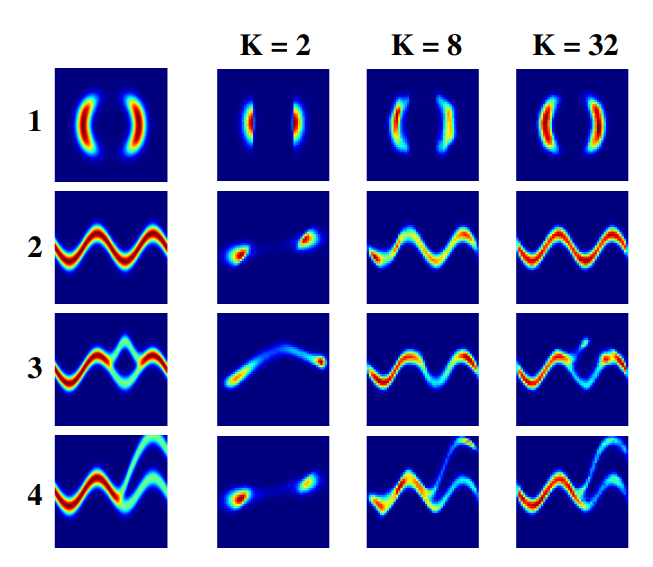
\includegraphics[width=0.3\textwidth]{Figures/ftvi/norm_flow_eg.png}
        \caption{\parencite{rezende2015variational} flows can transform a Gaussian into complex pushforward distributions}
    \end{figure}
\end{frame}

\begin{frame}
    \frametitle{Fat-tailed variational inference\footnote{\tiny \fullcite{liang2022fat}}}
    
    %%MM%% \textbf{Research aims (\cite{jaini2020tails}, this work)}: 
    %%MM%% What happens when $\pi$ is fat-tailed? What about when $\pi$ is multivariate?
    \textbf{Our Research Aims}:
    \begin{itemize}
        \item 
        What happens when $\pi$ is fat-tailed?
        \item 
        What about when $\pi$ is multivariate?
    \end{itemize}
    
    
    \begin{figure}[htbp]
      \centering
      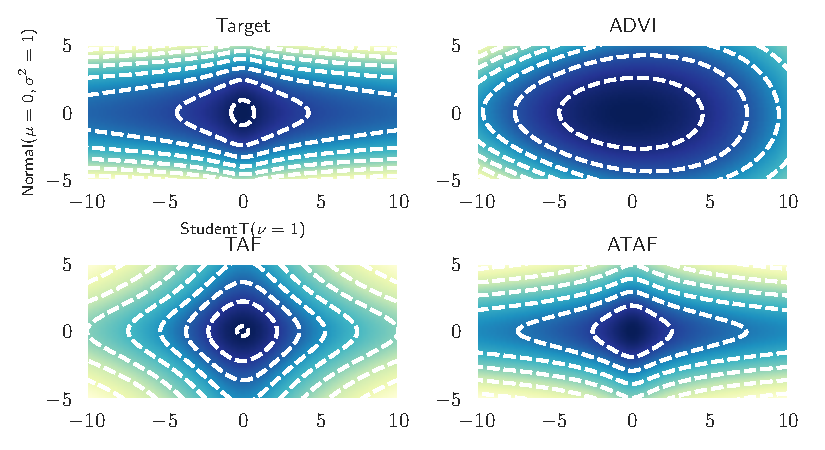
\includegraphics[width=0.7\textwidth]{Figures/ftvi/pancake.pdf}
      \label{fig:pancake}
    \end{figure}
\end{frame}

\begin{frame}{Methods}
    \textbf{Automatic Differentiation Variational Inference (ADVI, \cite{kucukelbir2017automatic,webb2019improving})}:
    
      \quad 
      $\cQ_\text{ADVI}~\coloneqq~\{
        (f_\theta)_\ast \mu
        \}$, 
      where $\mu = \text{Normal}(0_d, I_d)$.
      \vspace{3mm}
    \pause
    \textbf{Tail Adaptive Flows (TAF, \cite{jaini2020tails})}:
    
      \quad 
      $\cQ_\text{TAF}
        \coloneqq \{
        (f_\theta)_\ast \mu_\nu
        \}$,
      where $\mu_\nu = \prod_{i=1}^d \text{StudentT}(\nu)$ with $\nu \in \RR_+$.
      \vspace{3mm}
    \pause
    \textbf{Anisotropic Tail-Adaptive Flows (ATAF, this work)}:
    
      \quad 
      $\cQ_\text{ATAF}~\coloneqq~\{
        (f_\theta)_\ast \mu_{\vec{\nu}}
        \},$
      where $\mu_{\vec{\nu}} = \prod_{i=1}^d \text{StudentT}(\nu_i)$ with $\vec{\nu} \in \RR_+^d$.
\end{frame}

\subsection{Theory}

\begin{subframe}{Fat-tailed theory}
    \begin{definition}[Classification of tails]
        \label{def:tail-classification}
        For $\alpha,p > 0$, we let 
        \vspace{-1mm}
        \begin{itemize}
            \item $\mathcal{E}_\alpha^p$ denote the set of \emph{exponential-type} random variables $X$ with $\mathbb{P}(|X| \geq x) = \Theta(e^{-\alpha x^p})$ (e.g.
            $\overline{\cE_\alpha^2}$ are $\alpha^{-1/2}$-sub-Gaussians, $\overline{\cE_\alpha^1}$ are sub-exponentials).
        \vspace{-1mm}
            \item $\mathcal{L}_\alpha^p$ denote the set of \emph{logarithmic-type} random variables $X$ with $\mathbb{P}(|X| \geq x) = \Theta(e^{-\alpha(\log x)^p})$ (e.g.
            $\cL^1_\alpha$ are power laws)
        \end{itemize}
        \vspace{-1mm}
        Define the ascending families
        $\overline{\cE_\alpha^p}$ and $\overline{\cL_\alpha^p}$
        analogously as before except with $\Theta(\cdot)$ replaced
        by $\cO(\cdot)$.
    \end{definition}
\end{subframe}

\begin{frame}{Theoretical Result I}
    \begin{assumption}\label{assump:lipschitz}
        $f_\theta$ is invertible, and both $f_\theta$ and $f^{-1}_\theta$
        are $L$-Lipschitz continuous.
    \end{assumption}
    \pause
    \begin{theorem}
      \label{thm:distn_class_closed}
      \begin{itemize}[<+->]
          \item $f_\theta$ cannot make the tails of a fat-tailed distribution fatter (decrease tail parameter $\alpha$).
          \item If in addition $f_\theta$ is smooth with no critical points, then it cannot change
            the tail parameter of a fat-tailed distribution.
          \item Light-tailed distributions remain light-tailed under polynomial flows \parencite{jaini2019sum}.
      \end{itemize}
    \end{theorem}
\end{frame}

\subsubsection{Tail anisotropy}

\begin{frame}{Tail anisotropy}
    \begin{definition}[Tail anisotropy]
      \label{def:mv-tail-param}
      For random vector $X$, define
      $\alpha_X(v) = -\lim_{x \to \infty} \log \PP(\braket{v,X} \geq x) / \log x$ when the limit exists, and $\alpha_X(v) = +\infty$ otherwise.
      $X$ is \emph{tail-isotropic} if $\alpha_X(v) \equiv c < \infty$ is constant.
    \end{definition}

    \begin{figure}[htbp]
  \centering
  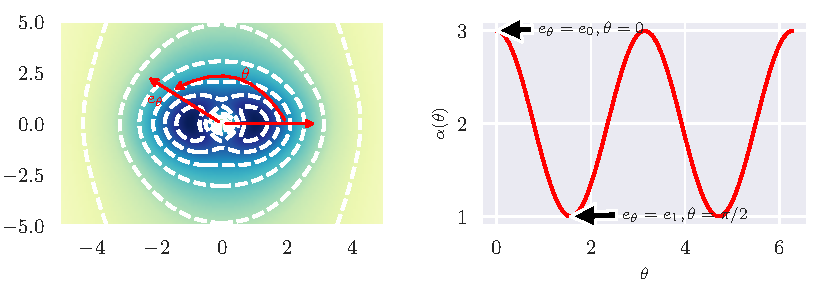
\includegraphics[width=0.85\textwidth]{Figures/ftvi/radial-fat-tail.pdf}%
%   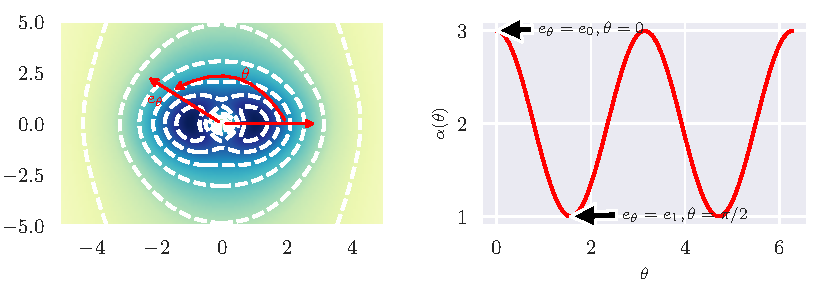
\includegraphics[trim={0 0 7cm 0},clip]{Figures/ftvi/radial-fat-tail.pdf}\\%
%   \vspace{-8mm}
%   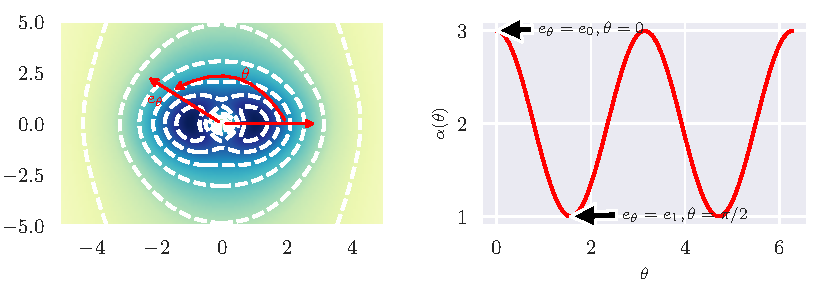
\includegraphics[trim={7.2cm 0 0 0},clip]{Figures/ftvi/radial-fat-tail.pdf}%
  %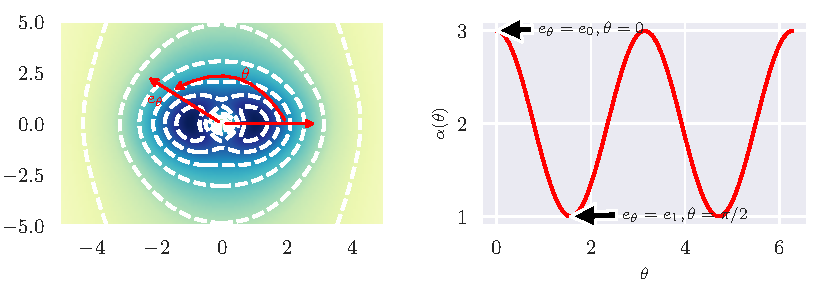
\includegraphics[width=\textwidth]{Figures/ftvi/radial-fat-tail.png}%
  %\input{Figures/ftvi/radial-fat-tail.pgf}
%   \caption{
%     A tail-anisotropic distribution with PDF $\dd P(r,\theta) = r^{-\alpha(\theta)} r \dd r \dd\theta$ (left)
%     and its tail-parameter function $\alpha(\theta) = 2 + \cos(2\theta)$ (right).
%   }
  \label{fig:radial-fat-tail}
\end{figure}
\end{frame}

% \begin{frame}{A problematic example}
%     \begin{figure}[htbp]
%     \centering
%     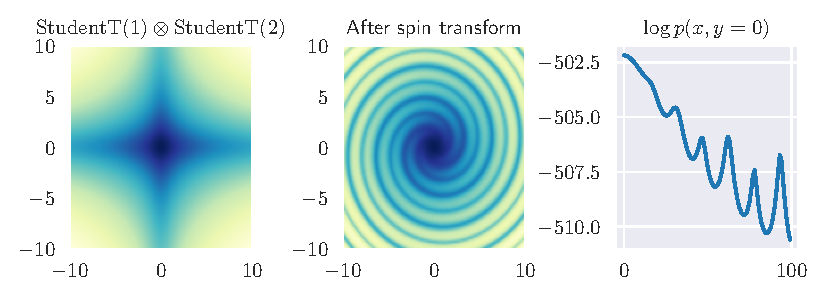
\includegraphics[width=\textwidth]{Figures/ftvi/spiral.pdf}
%     % 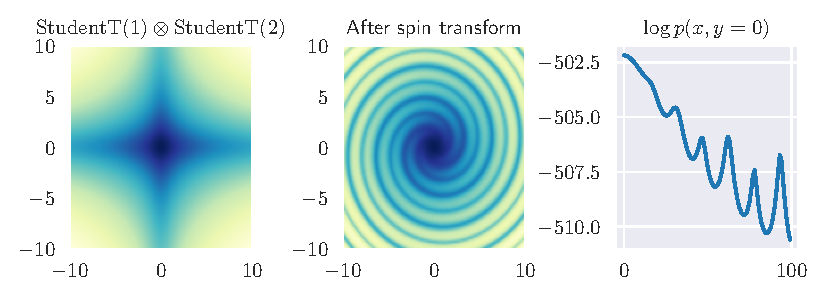
\includegraphics[trim={0 0 9cm 0},clip]{Figures/ftvi/spiral.pdf}\\
%     % 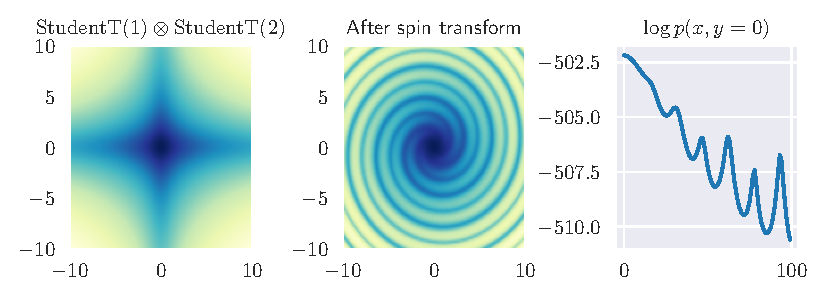
\includegraphics[trim={5cm 0 4.9cm 0},clip]{Figures/ftvi/spiral.pdf}\\
%     % 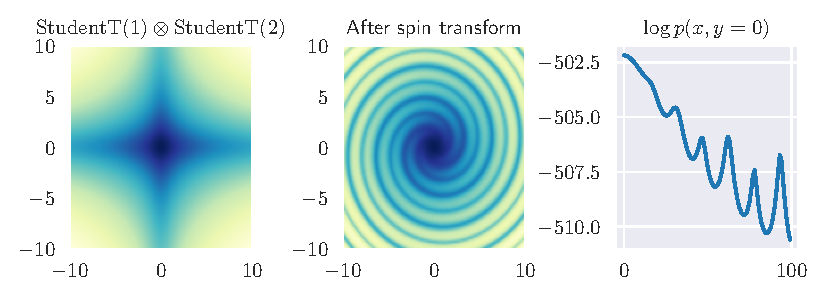
\includegraphics[trim={9.3cm 0 0cm 0},clip]{Figures/ftvi/spiral.pdf}\\

%     \label{fig:spiral}
% \end{figure}
% \end{frame}

\begin{frame}{Theoretical Result II}
    \begin{proposition}[Pushforwards of tail-isotropic distributions]
      \label{prop:isotropic-pushforward}
      Let $\mu$ be tail isotropic with non-integer parameter $\nu$
      and suppose $f_\theta$ satisfies \Cref{assump:lipschitz}.
      Then $(f_\theta)_\ast \mu$ is tail isotropic with parameter $\nu$.
    \end{proposition}
    
    \therefore\quad ATAF is necessary for anisotropic tails

    % \begin{remark}\label{remark:anisotropic}
    %   ATAF can represent tail-anisotropic distributions with up to $d$ different
    %   tail parameters while simultaneously satisfying \Cref{assump:lipschitz}.
    %   For example, if $\Phi_\text{Flow} = \text{Identity}$ and $\mu_\nu = \prod_{i=1}^d \text{StudentT}(i)$
    %   then the pushforward $(\Phi_\text{Flow})_\ast \mu_\nu = \mu_\nu$ is tail-anisotropic.
    %   % Moreover, its standard basis tail parameters are equal
    %   % (up to permutation) to those for $\mu$.
    % \end{remark}
\end{frame}

\subsection{Experiments}

\begin{subframe}{Bayesian linear regression}
\vspace{-10mm}
    \begin{gather*}
        \sigma^2 \sim \text{Inv-Gamma}(a_0, b_0)\\
        \beta \mid \sigma^2 \sim \cN(0, \sigma^2),\qquad
        y \mid X, \beta, \sigma \sim \cN(X \beta, \sigma^2) ,
    \end{gather*}
    
    The posterior is tail-anisotropic: 
    
    $p(\sigma^2, \beta=c \mid X, y) \propto \rho(\sigma^2) \in \cL^1_{\alpha_n}$ is fat-tailed (power-law)
    
    $p(\sigma^2=c, \beta \mid X, y) \propto \rho(\beta \mid c) \in \overline{\cE^2}$ is light-tailed (sub-Gaussian)

    % The posterior is tail-anisotropic since $p(\beta,\sigma^2 \mid X, y) = \rho(\sigma^2)\rho(\beta \mid \sigma)$ where $\rho(\beta \mid \sigma) = \cN(\Sigma_n(X^\top X \hat\beta), \sigma^2 \Sigma_n)$, $\Sigma_n = (X^\top X + \sigma^{-2})^{-1}$, $\hat\beta = (X^\top X)^{-1} X^\top y$, and
    % %\begin{align*}
    %     %p(\beta,\sigma^2 \mid X, y) &= \rho(\sigma^2) \rho(\beta \mid \sigma) \\
    %     \[
    %     \rho(\sigma^2) = \text{Inv-Gamma}\bigg(
    %     %\underbrace{a_0 + \frac{n}{2}}_{\eqqcolon a_n}, 
    %     a_0 + \frac{n}{2}, 
    %     b_0 + \frac{1}{2}(y^\top y - \mu_n^\top \Sigma_n \mu_n)\bigg). % \\
    %     \]
    %     %\rho(\beta \mid \sigma) &= \cN(\Sigma_n(X^\top X \hat\beta), \sigma^2 (X^\top X + \sigma^{-2} I)^{-1})
    % %\end{align*}
    % So for fixed $c$ we have that $p(\sigma^2, \beta=c \mid X, y) \propto \rho(\sigma^2) \in \cL^1_{\alpha_n}$
    % as a function of $\sigma$
    % and $p(\sigma^2=c, \beta \mid X, y) \propto \rho(\beta \mid c) \in \overline{\cE^2}$
    % as a function of $\beta$.
\end{subframe}

\begin{subframe}
    \begin{figure}[htbp]
  \centering
  \vspace{-0.2cm}
  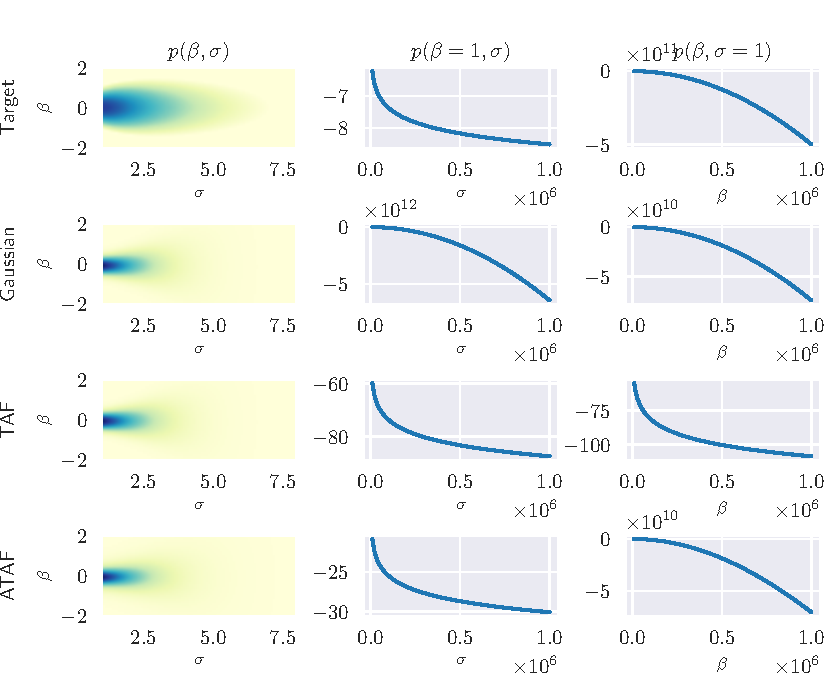
\includegraphics[width=0.75\textwidth]{Figures/ftvi/blr_aniso.pdf}
  \vspace{-0.3cm}
%   \caption{
%     Bayesian linear regression's tail-anisotropic posterior
%     (top left) exhibits a fat-tailed conditional in $\sigma$ (as evidenced by
%     the convex power-law decay in the top middle panel) and a Gaussian conditional in $\beta$ (concave graph in top right panel).
%     While all methods appear to provide a good approximation of the bulk (left column),
%     \Cref{prop:isotropic-pushforward} implies
%     Gaussian (Gaussian, second row) or isotropic StudentT product (TAF, third row) base distributions
%     yield Gaussian or power-law tails, respectively, for \emph{both} $\sigma$ and $\beta$.
%     In contrast, ATAF (bottom row) illustrates \Cref{remark:anisotropic} by
%     modeling simultaneously a power-law tail on $\sigma$ and Gaussian tail on $\beta$.
%   }
  \label{fig:blr-anisotropic}
\end{figure}
\end{subframe}


% \begin{subframe}{diamonds \cite{ghposteriordb}}
%     \begin{gather*}
%         \alpha \sim \text{StudentT}(\nu=3, \text{loc}=8, \text{scale}=10)\\
%         \sigma \sim \text{HalfStudentT}(\nu=3, \text{loc}=0, \text{scale}=10)\\
%         \beta \sim \cN(0, \mI_{24}),\qquad
%         y \sim \cN(\alpha + X \beta, \sigma) .
%     \end{gather*}

%     \begin{table}[htbp]
%         \centering
%         \begin{tabular}{rcc}
%             \tableheadrow
%                       & \tableheadcol{ELBO}                & \tableheadcol{$\log p(y)$}       \\
%             ADVI      & $\mathbf{2873.90} \pm 6.95$    & $2969.73 \pm 1.73$ \\
%             TAF       & $2839.64 \pm 9.10$    & $2973.85 \pm 0.87$ \\
%             ATAF      & $2842.75 \pm 8.83$    & $\mathbf{2976.75} \pm 0.66$ \\
%             \hline
%             NUTS      & n/a                  & $3724.59 \pm 0.036$ \\
%         \end{tabular}
%         %\caption{diamonds}
%         \label{tab:diamonds}
%     \end{table}
% \end{subframe}

\begin{frame}{Eight schools \parencite{rubin1981estimation}}
    \begin{gather*}
        \tau \sim \text{HalfCauchy}(\text{loc}=0, \text{scale}=5)\\
        \mu \sim \cN(0, 5),\qquad
        \theta \sim \cN(\mu, \tau),\qquad
        y \sim \cN(\theta, \sigma) .
    \end{gather*}

    \begin{table}[htbp]
        \centering
        \begin{tabular}{rcc}
            \toprule
                      & ELBO                & $\log p(y)$       \\
            \midrule
            ADVI      & $-72.13 \pm 6.89$    & $-53.25 \pm 3.44$ \\
            TAF       & $-64.64 \pm 4.88$    & $-52.51 \pm 4.41$ \\
            ATAF      & $\mathbf{-58.63} \pm 4.75$    & $\mathbf{-51.01} \pm 3.71$ \\
            \hline
            NUTS      & n/a                  & $-47.78 \pm 0.093$ \\\bottomrule
        \end{tabular}
        %\caption{Eight schools}
        \label{tab:eight_schools}
    \end{table}
\end{frame}

\begin{frame}{Financial \parencite{fama2015five} and actuarial \parencite{cms} density modeling}
    \begin{table}[htbp]
    \centering
    \begin{tabular}{rcc}
        \toprule
                  & Fama-French 5 Industry Daily & CMS 2008-2010 DE-SynPUF       \\
        \midrule
        ADVI      & $-5.018 \pm 0.056$    & $-1.883 \pm 0.012$ \\
        TAF       & $-4.703 \pm 0.023$    & $-1.659 \pm 0.004$ \\
        ATAF      & $\mathbf{-4.699} \pm 0.024$    & $\mathbf{-1.603} \pm 0.034$ \\\bottomrule
    \end{tabular}
    \vspace{-2mm}
    \caption{
        Log-likelihoods (higher is better, $\pm$ standard errors).
    }
    \label{tab:density-estimation}
\end{table}
\end{frame}

% \subsection{Conclusion}

% \begin{frame}{Conclusions}
%     \begin{itemize}[<+->]
%         \item Tails of flow-based variational approximations are limited by choice of base distribution!
%         \item 
%         %%MM%% Prior work (TAF, \cite{jaini2020tails}) considers univariate tails, and in this work:
%         We improved prior work (TAF, \cite{jaini2020tails}), which considered univariate tails, in the following ways:
%         \begin{itemize}
%             \item 
%             Prior univariate theory is refined to include $\alpha$ and
%             closure results are sharpened
%             \item 
%             A multivariate theory is proposed to quantify tail-anisotropy and prove
%             ATAF's necessity
%             \item 
%             Experiments confirm ATAF's improvements on real-world fat-tailed datasets
%         \end{itemize}
%     \end{itemize}
% \end{frame}

\section{Generalized Gamma Algebra for Fat Tails}

\begin{frame}{High-level Idea}
    \begin{figure}
        \centering
        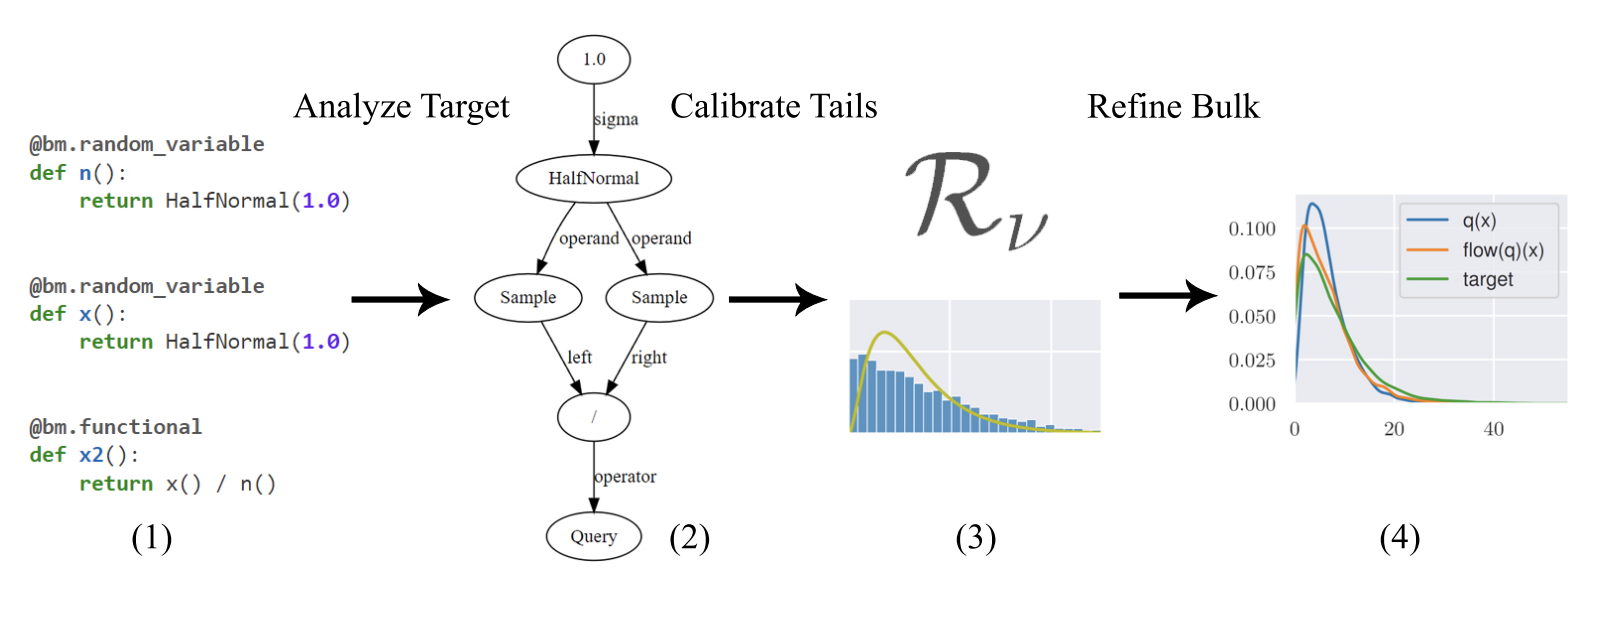
\includegraphics[width=1\textwidth]{Figures/gga/schematic.png}
    \end{figure}
\end{frame}

\begin{frame}{Generalized gamma tail parameterization}
    \begin{definition}
        Let $\nu \in \mathbb{R}$, $\sigma > 0$, and $\rho \in \mathbb{R} \backslash \{0\}$ be such that $(\nu+1)/ \rho > 0$.
        A non-negative random variable $X$ is \emph{generalized Gamma distributed} with parameters $\nu,\sigma,\rho$ if it has Lebesgue density
        \begin{equation}
        \label{eq:GenGammaDensity}
        p_{\nu,\sigma,\rho}(x) = c_{\nu,\sigma,\rho} x^\nu e^{-\sigma x^\rho},\qquad x > 0,
        \end{equation}
        where $c_{\nu,\sigma,\rho} = \rho \sigma^{(\nu+1)/\rho} / \Gamma((\nu+1)/\rho)$ is the normalizing constant. %The generalized Gamma density incorporates many other well-known densities, including that of the Gamma distribution ($\rho = 1$), and the Frechet/Weibull distribution ($\nu = \rho - 1$). 
    \end{definition}
\end{frame}

\begin{subframe}{Static analysis in PPL}
    \begin{algorithm}[H]
    	\caption{Pseudocode for a GGA tails static analysis pass}\label{alg:bfs_typecheck}
    	\KwData{Abstract syntax tree for a PPL program}
    	\KwResult{GGA parameter estimates for all random variables}
    	frontier $\gets$ [rv : Parents(rv) = $\emptyset$]\;
    	GGAs $\gets \{\}$\;
    	\While{\text{frontier} $\neq \emptyset$}{
    		next $\gets$ frontier.popLeft()\;
    		GGAs[next] $\gets$ computeGGA(next.op, next.parent)\;
    		frontier $\gets$ frontier + next.children()\;
    	}
    	\Return{GGAs}
    \end{algorithm}
\end{subframe}

\begin{frame}{Prior work \parencite{resnick2007heavy}: closure under addition}
    \begin{align*}
        &  (\nu_{1},\sigma_{1},\rho_{1})\oplus(\nu_{2},\sigma_{2},\rho_{2}) \\
        & \equiv \begin{cases}
            \max\{(\nu_{1},\sigma_{1},\rho_{1}),(\nu_{2},\sigma_{2},\rho_{2})\} & \text{ if }\rho_{1}\neq\rho_{2}\text{ or }\rho_{1},\rho_{2}<1\\
            \left(\nu_{1}+\nu_{2}+1,\min\{\sigma_{1},\sigma_{2}\},1\right) & \text{ if }\rho_{1}=\rho_{2}=1\\
            (\nu_{1}+\nu_{2}+\frac{2-\rho}{2},(\sigma_{1}^{-\frac{1}{\rho-1}}+\sigma_{2}^{-\frac{1}{\rho-1}})^{1-\rho},\rho) & \text{ if }\rho=\rho_{1}=\rho_{2}>1.
        \end{cases}
    \end{align*}
\end{frame}

\begin{frame}{New: closure under multiplication\footnote{\fullcite{gga}}}
    \begin{align*}
        & (\nu_{1},\sigma_{1},\rho_{1})\otimes(\nu_{2},\sigma_{2},\rho_{2}) \\
        &\qquad \equiv\begin{cases}
        \left(\frac{1}{\mu}\left(\frac{\nu_{1}}{|\rho_{1}|}+\frac{\nu_{2}}{|\rho_{2}|}+\frac{1}{2}\right),\sigma,-\frac{1}{\mu}\right) & \text{ if }\rho_{1},\rho_{2}<0\\
        \left(\frac{1}{\mu}\left(\frac{\nu_{1}}{\rho_{1}}+\frac{\nu_{2}}{\rho_{2}}-\frac{1}{2}\right),\sigma,\frac{1}{\mu}\right) & \text{ if }\rho_{1},\rho_{2}>0\\
        \mathcal{R}_{|\nu_1|} & \mbox{ if }\rho_{1}\leq0,\rho_{2}>0 \\
        \mathcal{R}_{\min\{|\nu_1|,|\nu_2|\}} & \mbox{ if }\rho_{1}=0,\rho_{2}=0
        \end{cases} \\
        &\text{where }\mu=\frac{1}{|\rho_{1}|}+\frac{1}{|\rho_{2}|}=\frac{|\rho_{1}|+|\rho_{2}|}{|\rho_{1}\rho_{2}|}, \sigma=\mu(\sigma_{1}|\rho_{1}|)^{\frac{1}{\mu|\rho_{1}|}}(\sigma_{2}|\rho_{2}|)^{\frac{1}{\mu|\rho_{2}|}}.
    \end{align*}
\end{frame}

\begin{frame}{New: closure under Lipschitz maps, bulk correction}
    \begin{align*}
        & f(X_1,\dots,X_n) \equiv L \max\{X_1,\dots,X_n\}
    \end{align*}
    \begin{figure}
        \centering
        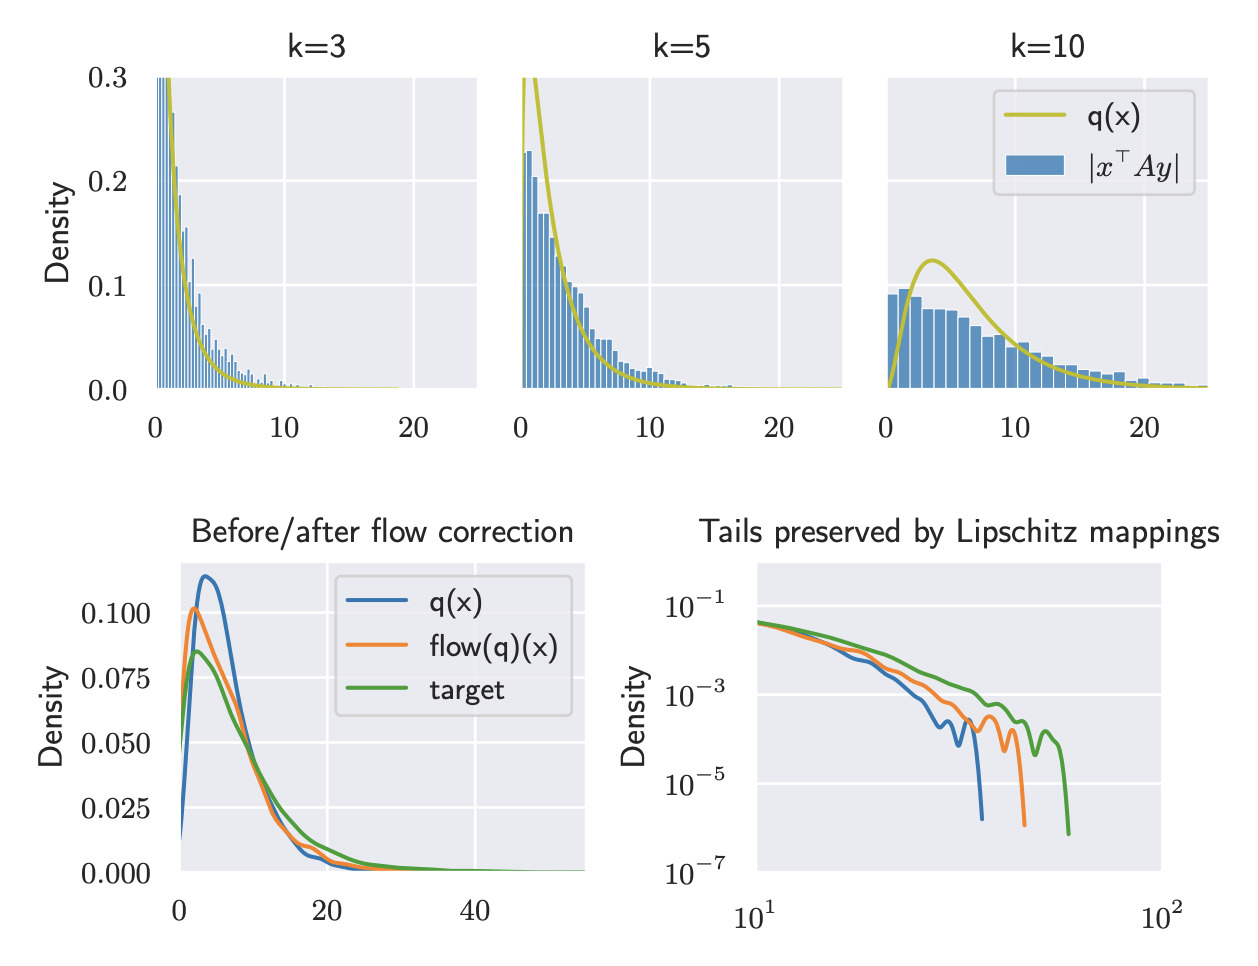
\includegraphics[width=0.7\textwidth]{Figures/gga/flow-correction.png}
    \end{figure}
\end{frame}

\begin{frame}{Results: variational inference}
    \begin{figure}
        \centering
        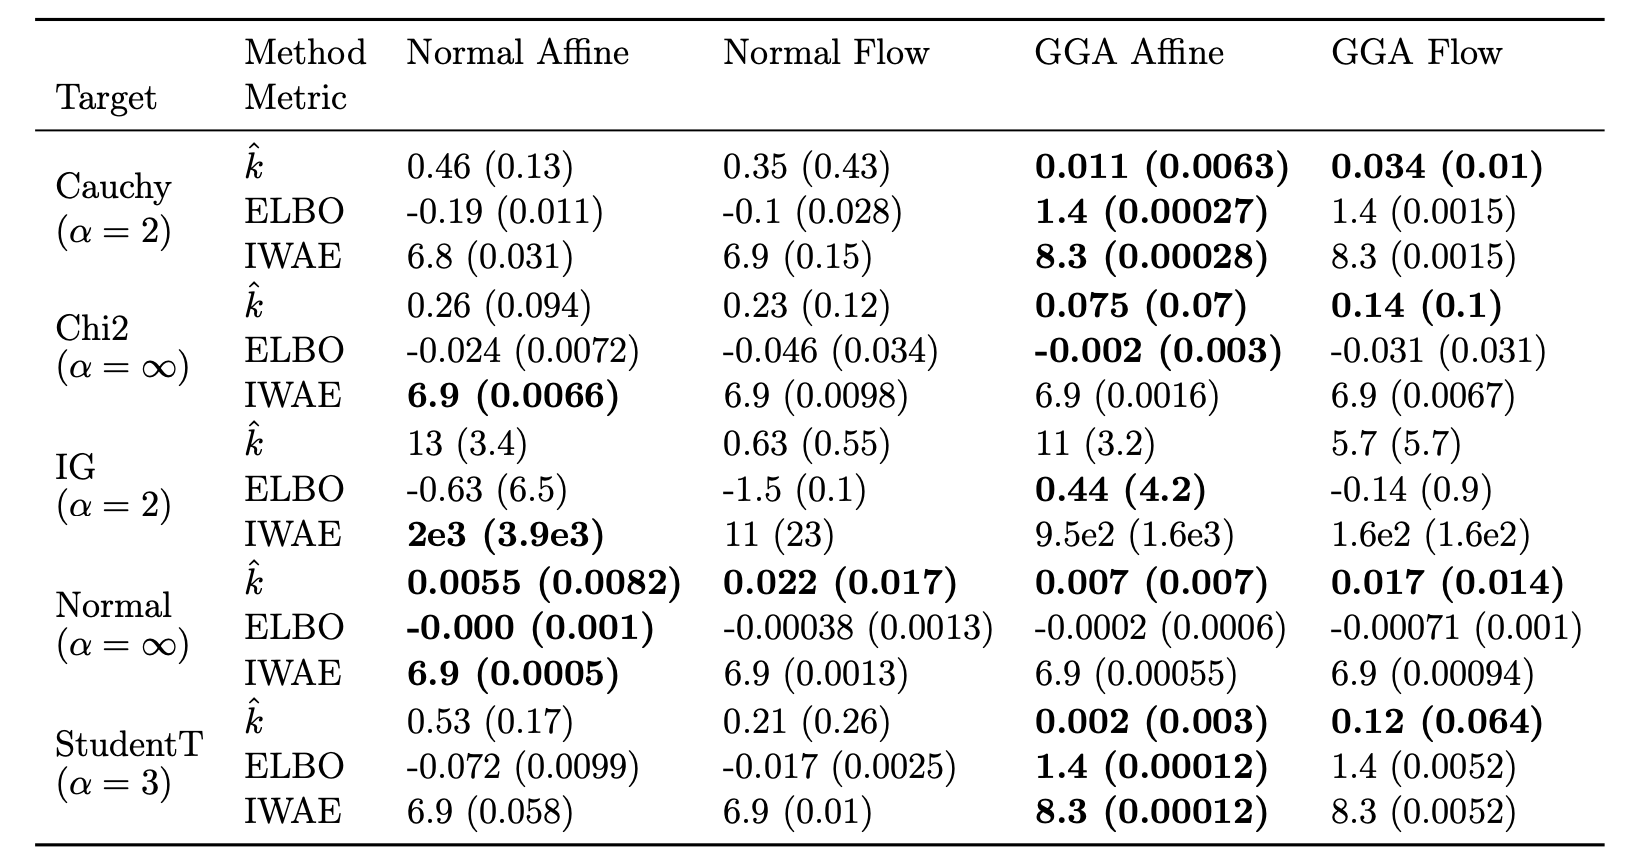
\includegraphics[width=\textwidth]{Figures/gga/vi.png}
    \end{figure}
\end{frame}

\begin{frame}{Results: density estimation}
    \begin{figure}
        \centering
        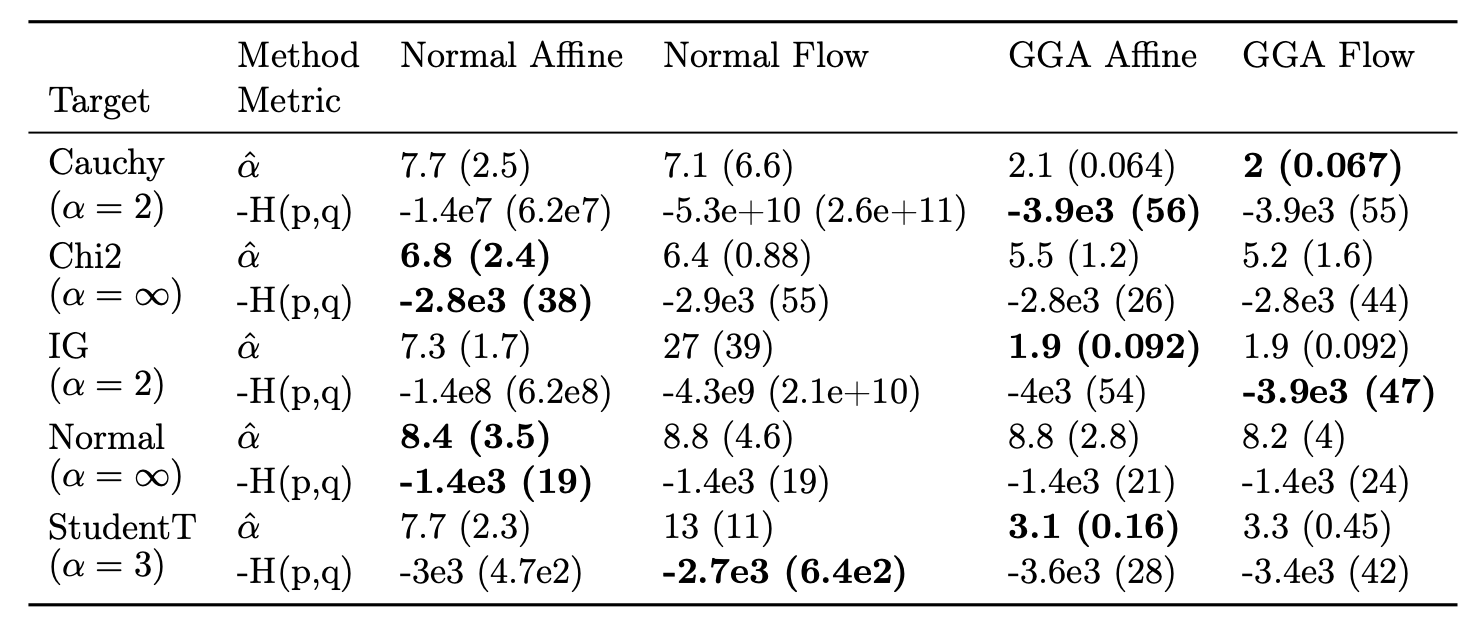
\includegraphics[width=\textwidth]{Figures/gga/de.png}
    \end{figure}
\end{frame}

% \section{Lightweight Inference Compilation}

% \subsection{Background on Probabilistic Programming}

\begin{subframe}[fragile]{Probabilistic programming languages}

\begin{quote}
    Just as programming beyond the simplest algorithms requires tools for abstraction and composition, complex probabilistic modeling requires new progress in model representation—probabilistic programming languages.
\end{quote}
\parencite{goodman2013principles}
\end{subframe}

\begin{subframe}[fragile]{Abstractions over deterministic computations}
\begin{minipage}{0.4\linewidth}
    \begin{lstlisting}[language={[x86masm]Assembler}] 
mov  dx, msg
; ah=9 - "print string" sub-function
mov  ah, 9
int  0x21

"terminate program" sub-function
mov  ah, 0x4c
int  0x21

msg  db 'Hello, World!', 0x0d, 0x0a, '$'
    \end{lstlisting}
\end{minipage}$\iff$
\begin{minipage}{0.48\linewidth}
    \begin{lstlisting}[language=python]
    print("Hello, World!")
    \end{lstlisting}
\end{minipage}
\note[itemize]{
\item Familiar: Abstraction / composition over assembly code, deterministic computations
\item Easier to understand, debug, maintain; compiler can optimize as long as results consistent
\item Same benefits for PPLs, but now for stochastic computations (reasoning under uncertainty)
}
\end{subframe}

% \begin{frame}[fragile]{Abstractions over probabilistic computations}
\begin{frame}[fragile]{Probabilistic programming languages}
\begin{minipage}{0.4\linewidth}
    \begin{figure}
        \centering
        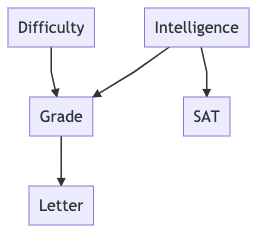
\includegraphics[width=\linewidth]{Figures/lic/student-network.png}
        \caption{Student scenario, \parencite{koller2009probabilistic}}
    \end{figure}
% graph TD
%   D[Difficulty] --> G[Grade]
%   I[Intelligence] --> G
%   I --> S[SAT]
%   G --> L[Letter]
\end{minipage}
\pause
\begin{minipage}{0.58\linewidth}
    \begin{verbatim}
    d ~ dPrior
    i ~ iPrior
    g ~ gCond(d, i)
    s ~ sCond(i)
    l ~ lCond(g)
    \end{verbatim}
\end{minipage}

\pause

\textbf{Example Query}: \texttt{infer(i, {l=Good, s=800})}

Given a student's recommendation \emph{letter} and \emph{SAT} score,
what should I expect their \emph{intelligence} to be?


\note[itemize]{
    \item Probabilistic model for student recommendation letters and SAT scores
    \item Priors and conditionals
    \item Observations (Letter, SAT), Queries (Intelligence)
}
\end{frame}

\begin{frame}[fragile]{Monte Carlo approximation}
\begin{align*}
    &\mathbb{E}[\text{Intelligence} | \text{Letter}=\text{Good}, \text{SAT}=1600] \\
    &= \int I \cdot \Pr[\text{Intelligence}=I | \text{Letter}=\text{Good}, \text{SAT}=1600] dI \\
    &\approx \frac{1}{N} \sum_{n=1}^N I_n
\end{align*}
where $I_n \overset{\text{iid}}{\sim} \Pr[\text{Intelligence} | \text{Letter}=\text{Good}, \text{SAT}=1600]$

\note[itemize]{
\item Integrals are just really tiny sums, CLT $1/\sqrt{N}$ rate
\item Can answer this question by drawing samples from the posterior, inference is solved by sampling the posterior
}
\end{frame}

\begin{frame}[fragile]{Monte Carlo Markov Chain}
    How to sample? Consider producing $\{I_n\}$ by:
    \begin{itemize}
        \item Fix $\text{Letter}=\text{Good}$ and $\text{SAT}=1600$
        \item Repeat:
        \begin{itemize}[<+->]
            \item UAR choose a latent variable to resample
            \item Sample a \emph{proposal distribution} $Q(\cdot)$ to propose a new value
            \item Accept with probability $\alpha$ and revert otherwise, emit $I_n$
        \end{itemize}
    \end{itemize}
    \pause
    \begin{theorem}[\cite{hastings1970monte}]
        With appropriately chosen $\alpha$, the above algorithm yields
        a Markov Chain with the posterior as the invariant distribution.
    \end{theorem}
\end{frame}

\subsection{Inference Compilation}

\begin{frame}[fragile]{Proposal distributions}
    Different $Q(\cdot)$ $\implies$ different MCMC algorithms
    
    \begin{itemize}
        \item Random walk MH: $Q(\cdot)$ isotropic Gaussian
        \item Newtonian Monte Carlo \parencite{arora2020newtonian}:
        $Q(\cdot) =$ Hessian-based Gaussian
        \item Hamiltonian Monte Carlo: $Q(\cdot)$ integrates dynamical system
        \item \emph{Inference Compilation}: $Q(\cdot)$ output of a neural network
    \end{itemize}
\end{frame}

\begin{frame}{Intuition for IC}
    \begin{figure}
        \centering
        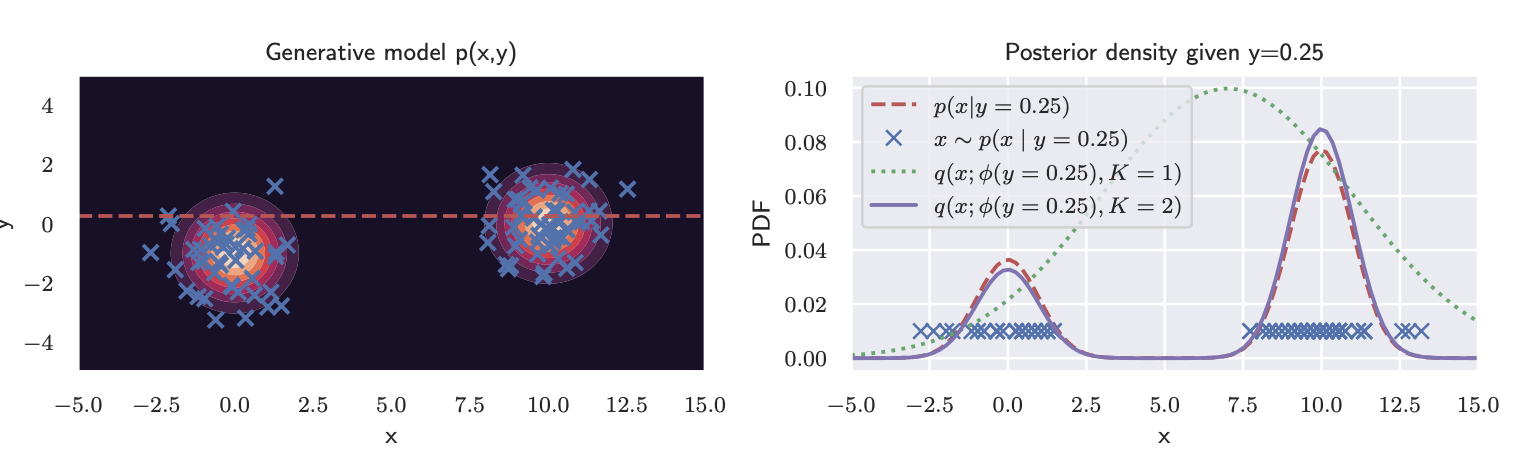
\includegraphics[width=\textwidth]{Figures/lic/intuition.png}
    \end{figure}
\end{frame}

% \begin{frame}[fragile]{Prior work: IC in imperative PPLs}
% 	\begin{figure}
% 	    \centering
% 	    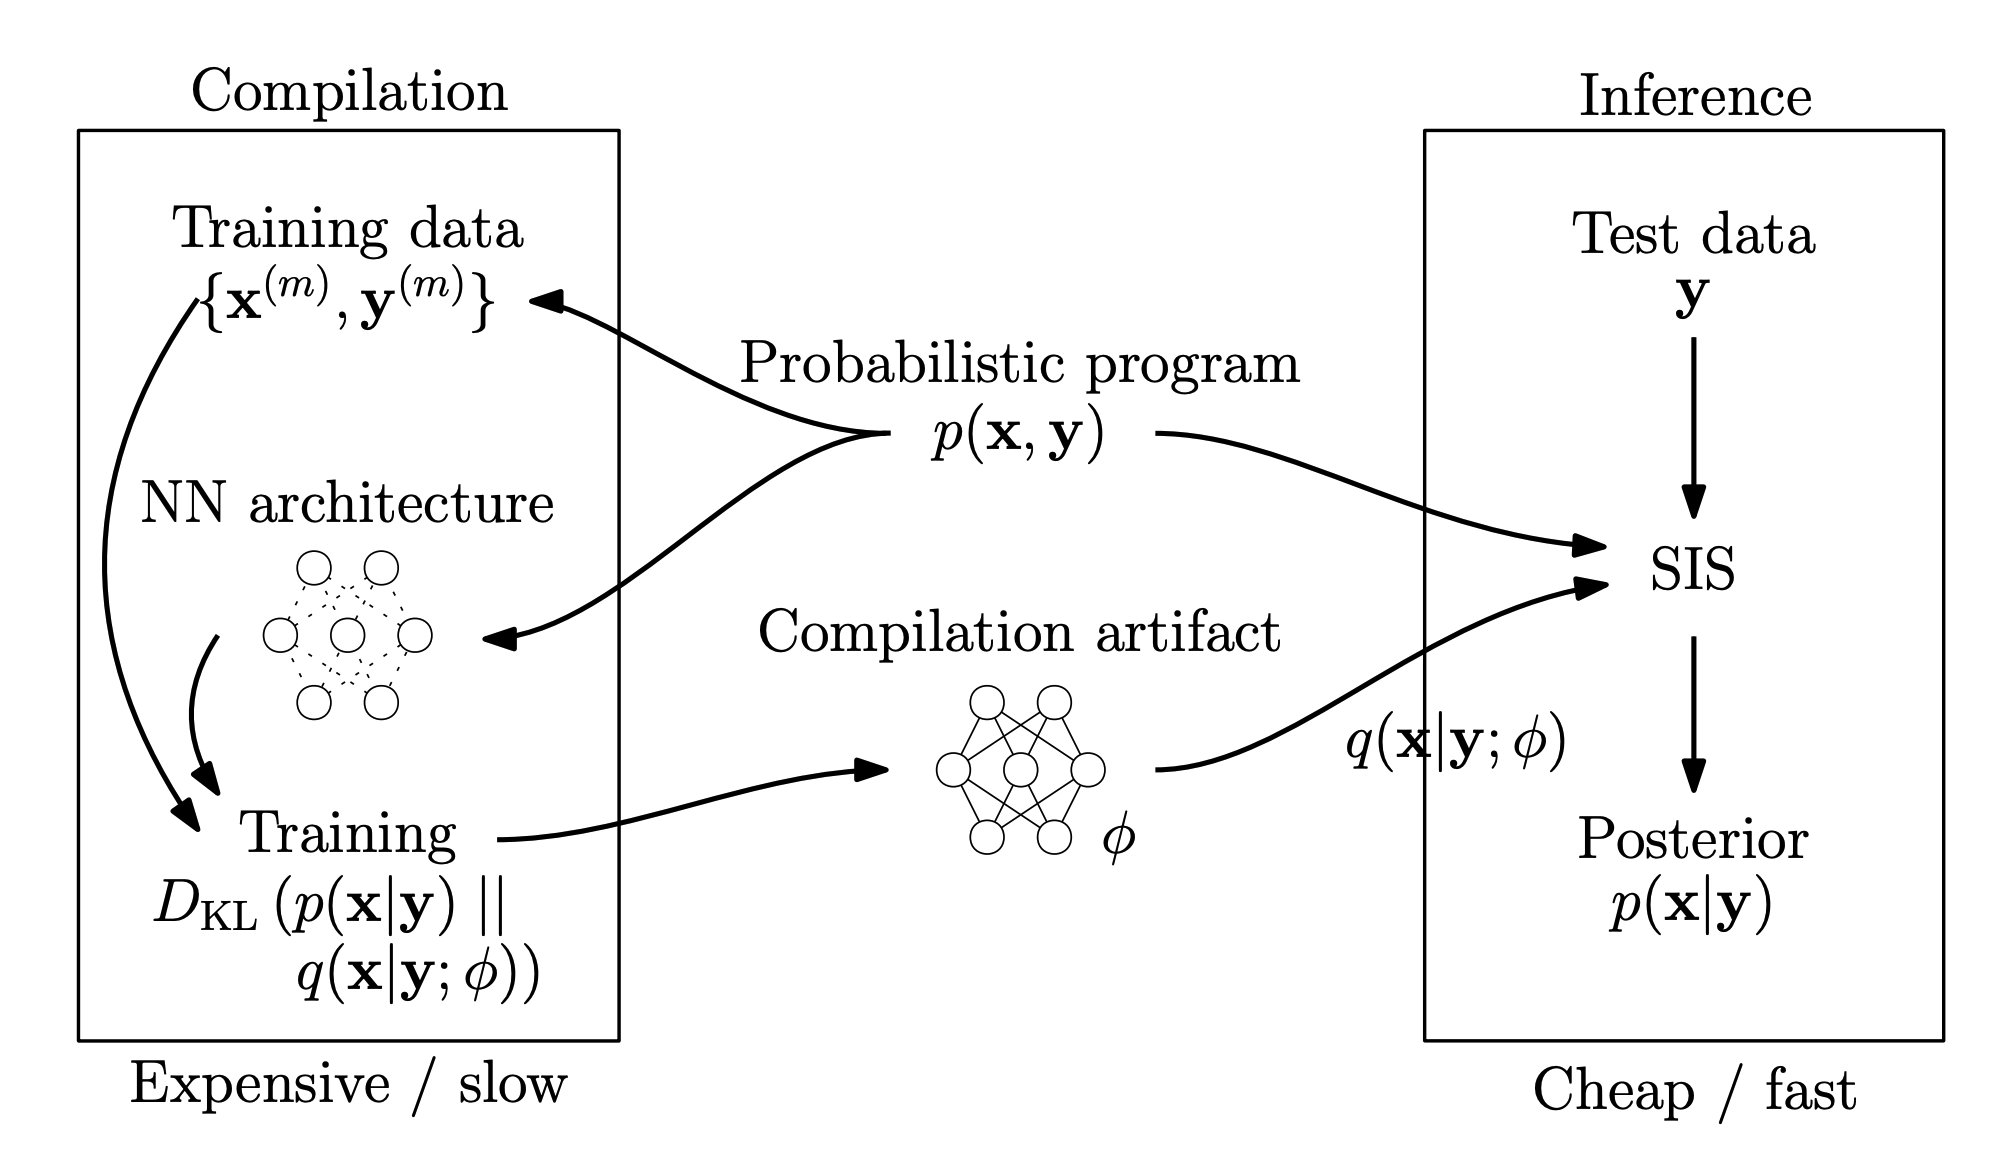
\includegraphics[width=0.7\linewidth]{Figures/lic/ic.png}
% 	    \caption{Inference compilation in SMC \cite{le2017inference}}
% 	\end{figure}
	
% 	\note[itemize]{
% 	\item Similar
% 	\begin{itemize}
% 	    \item Forward sampling of PP to generate training data
% 	    \item Minimize inclusive KL MC estimate from generated data
% 	    \item Amortize IC artifacts across many observations $\vec{y}$
% 	\end{itemize}
% 	\item Differences
% 	\begin{itemize}
% 	    \item SIS vs MH, minimal I-map
% 	\end{itemize}
% 	}
% \end{frame}

\begin{frame}[fragile]{Prior Work: Trace-based IC \parencite{le2017inference}}
\begin{minipage}{0.4\linewidth}
    \begin{figure}
        \centering
        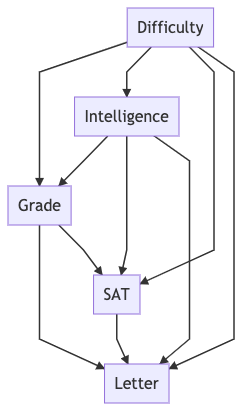
\includegraphics[width=\linewidth]{Figures/lic/student-network-smc-ic.png}
    \end{figure}
% graph TD
%   D[Difficulty] --> G[Grade]
%   D --> I
%   D --> S
%   D --> L
%   I[Intelligence] --> G
%   I --> S[SAT]
%   I --> L
%   G --> L[Letter]
%   G --> S
%   S --> L
\end{minipage}
\begin{minipage}{0.5\linewidth}
    \begin{align*}
        & q(d | \text{observations}) \\
        & q(i|d, \text{observations}) \\
        & q(g | i, d, \text{observations}) \\
        & q(s | g, i, d, \text{observations}) \\
        & q(l | s, g, i, d, \text{observations})
    \end{align*}
\end{minipage}
\end{frame}

\begin{frame}[fragile]{Our contribution: IC with minimal I-maps\footnote{\fullcite{liang2021accelerating}}}
    \begin{minipage}{0.4\linewidth}
    \begin{figure}
        \centering
        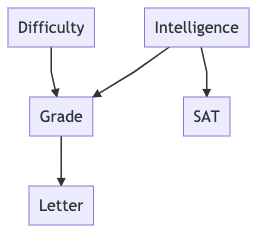
\includegraphics[width=\linewidth]{Figures/lic/student-network.png}
    \end{figure}
\end{minipage}
\begin{minipage}{0.5\linewidth}
\begin{align*}
    & q(d | g, i, \text{observations}) \\
    & q(i | g, d, s, \text{observations}) \\
    & q(g | i, d, l, \text{observations}) \\
    & q(s | i, \text{observations}) \\
    & q(l | g, \text{observations})
\end{align*}
\end{minipage}
    \note[itemize]{
    \item Each IC proposer only has access to Markov Blanket, respects causal structure
    \item SIS IC suffers in presence of nuisance parameters, requires attention to perform well
    \item Explain declarative vs imperative (parents are clearly demarcated)
    }
\end{frame}


\begin{frame}{Architecture}
    \begin{figure}
        \centering
        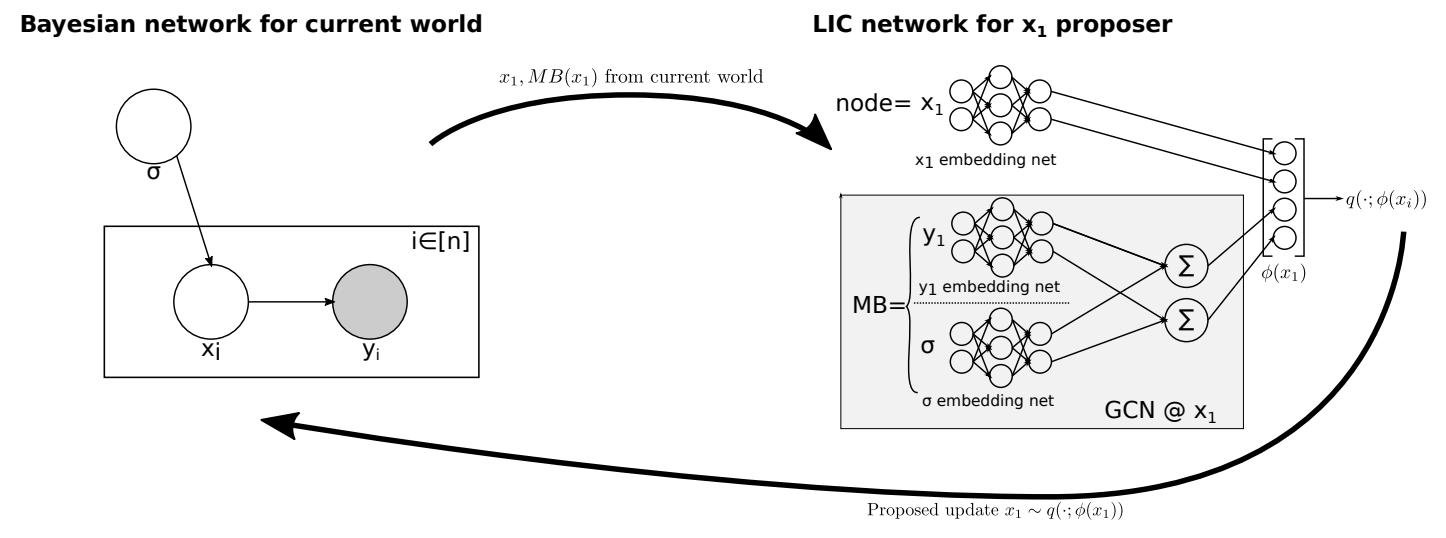
\includegraphics[width=\textwidth]{Figures/lic/schematic-eg.png}
    \end{figure}
    
    ``Deep sets'' \parencite{zaheer2017deep} applied to Markov Blanket
\end{frame}


\begin{frame}[fragile]{Example IC proposer for "grade"}

\begin{figure}
    \centering
    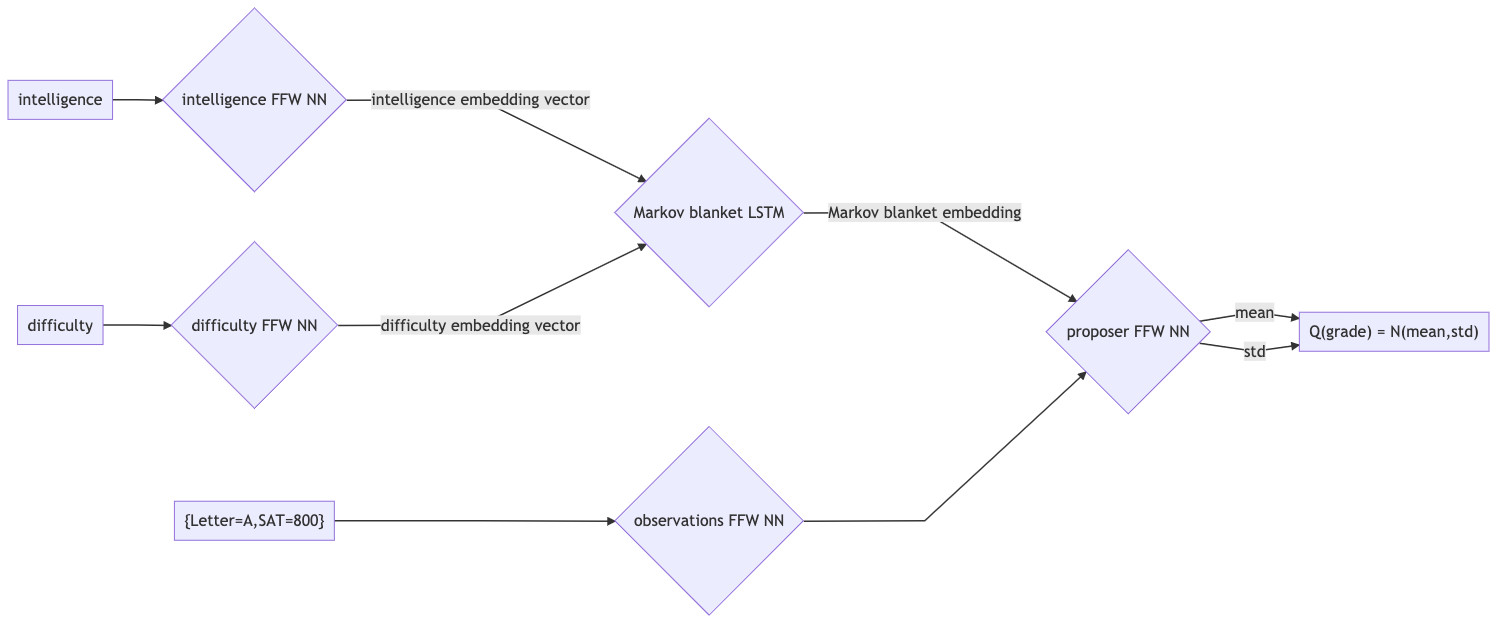
\includegraphics[width=\linewidth]{Figures/lic/ic-grade.png}
    \caption{IC proposer for \texttt{grade}}
% graph LR
% 	O["{Letter=A,SAT=800}"] --> Oe{observations FFW NN}
%   I[intelligence] --> Ie{intelligence FFW NN}
%   D[difficulty] --> De{difficulty FFW NN}
% 	Ie -->|intelligence  embedding vector| MB{Markov blanket LSTM}
%   De -->|difficulty embedding vector| MB
%   MB -->|Markov blanket embedding| P{proposer FFW NN}
%   Oe --> P
%   P -->|mean| Q["Q(grade) = N(mean,std)"]
%   P -->|std| Q
\end{figure}

\note[itemize]{
    \item Markov blanket can change size due to switching variables => LSTM
    \item Problem: density estimator currently Gaussian/Categorical
    \item Problem: observations shape fixed at compile
}
\end{frame}


\subsection{Results}

\begin{frame}{Results: GMM mode escape}
    \begin{figure}
        \centering
        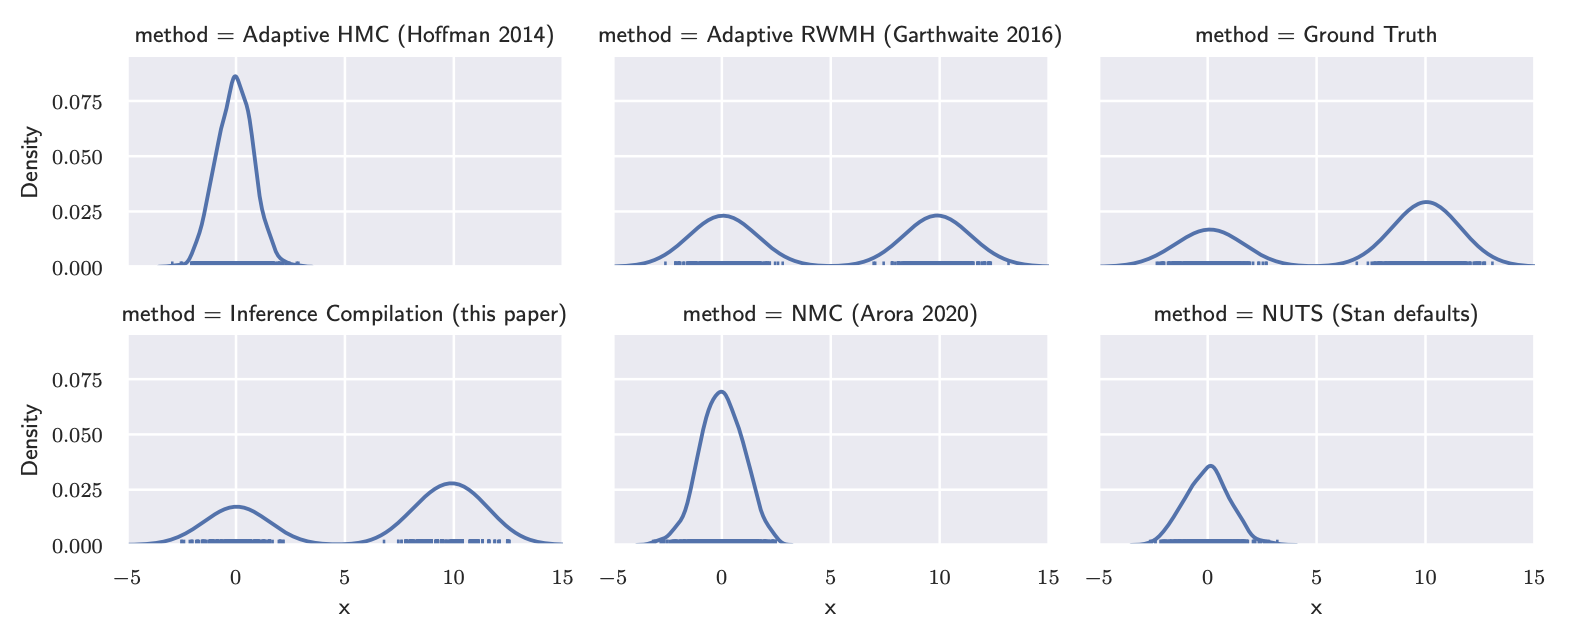
\includegraphics[width=\textwidth]{Figures/lic/gmm-escape.png}
    \end{figure}
\end{frame}

\begin{frame}{Results: nuisance parameter robustness}
    \begin{figure}[p]
        \centering
        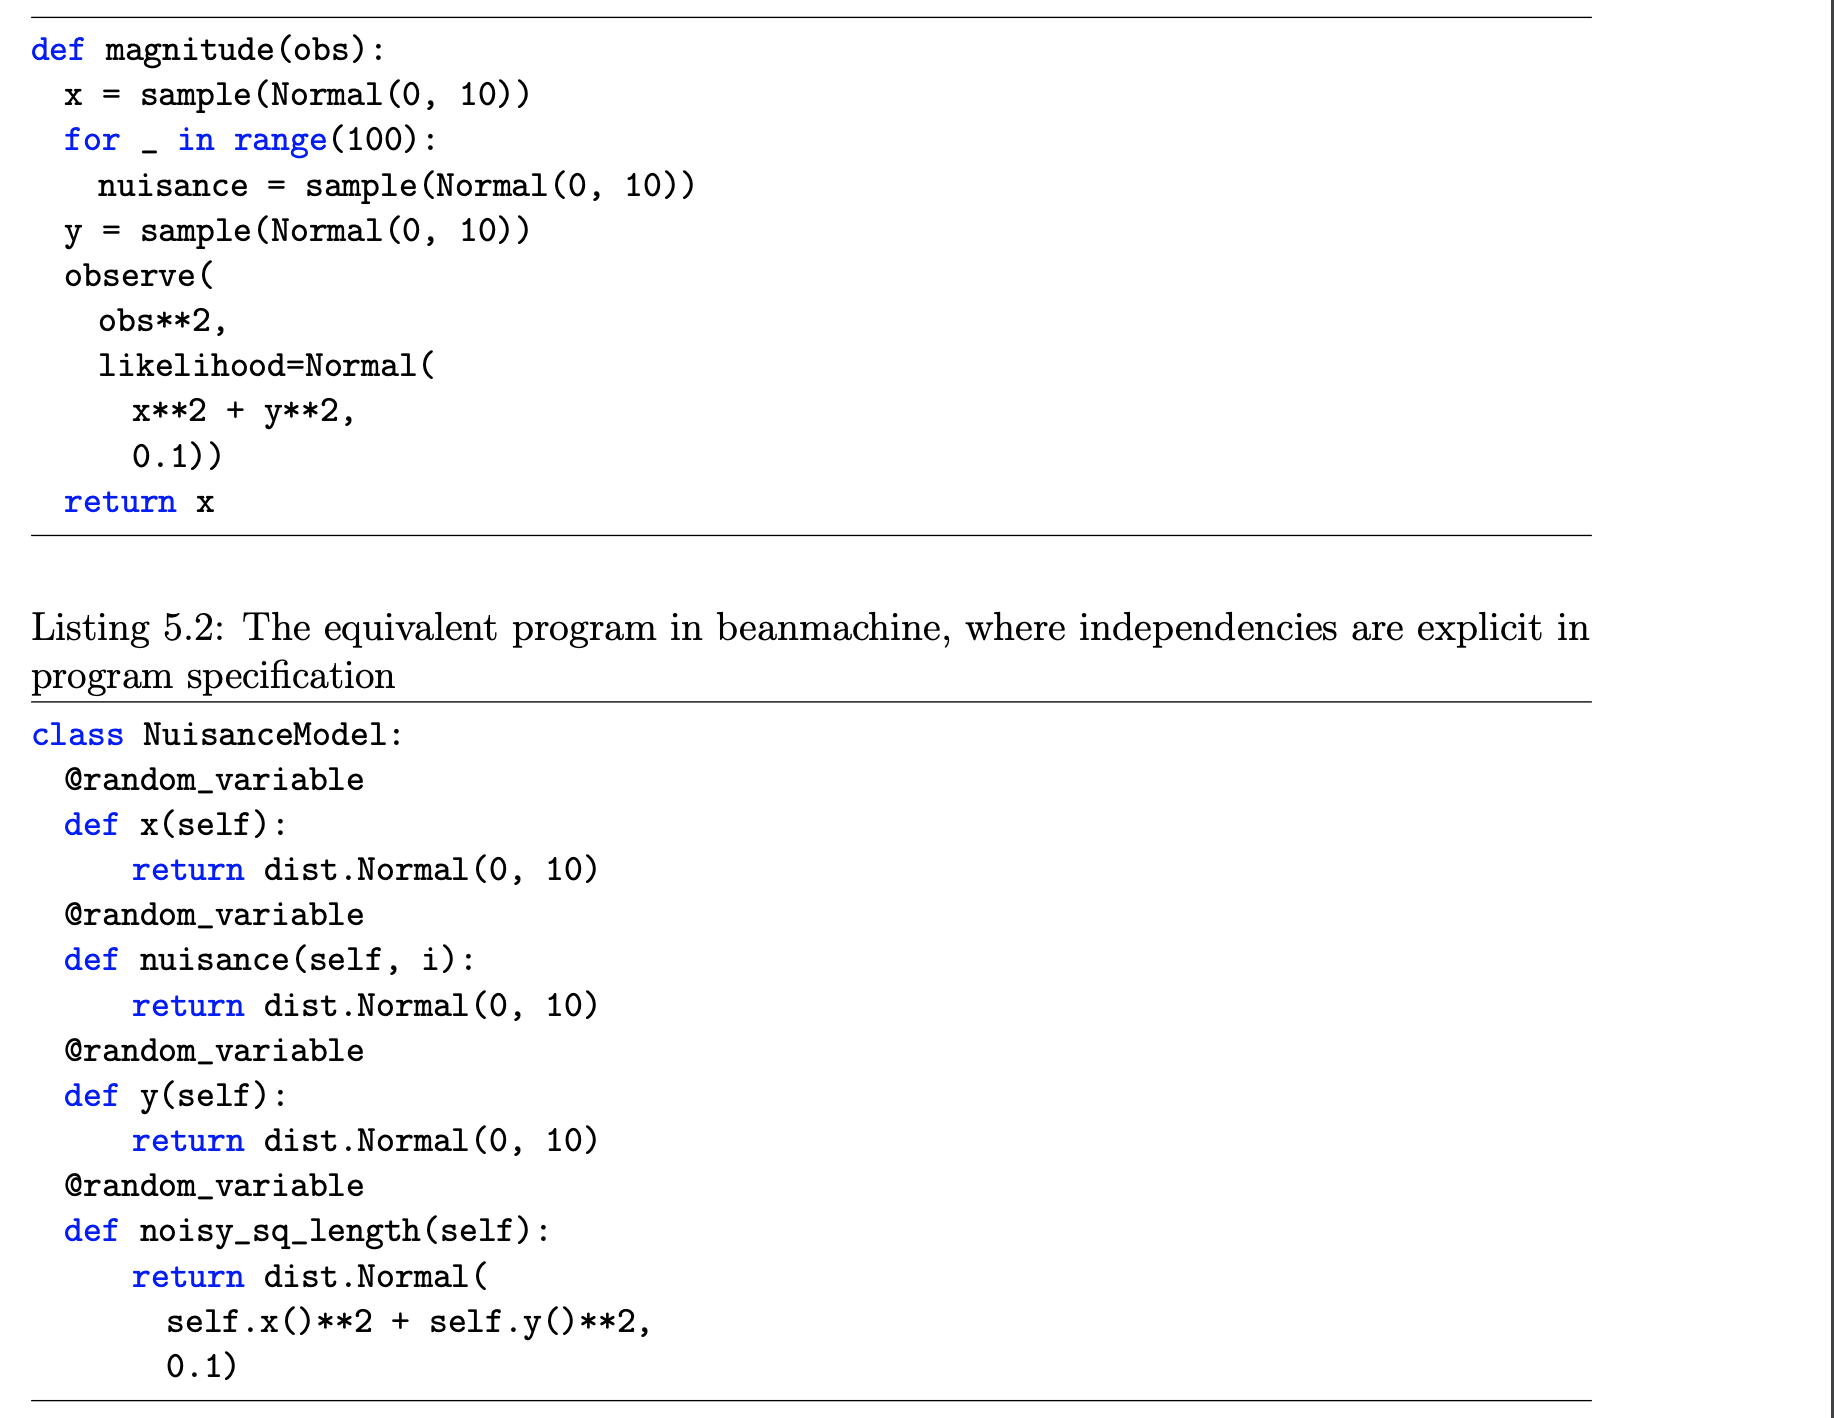
\includegraphics[width=0.4\textwidth,trim={0 16cm 20cm 0.5cm},clip]{Figures/lic/nuisance-progs.png}
        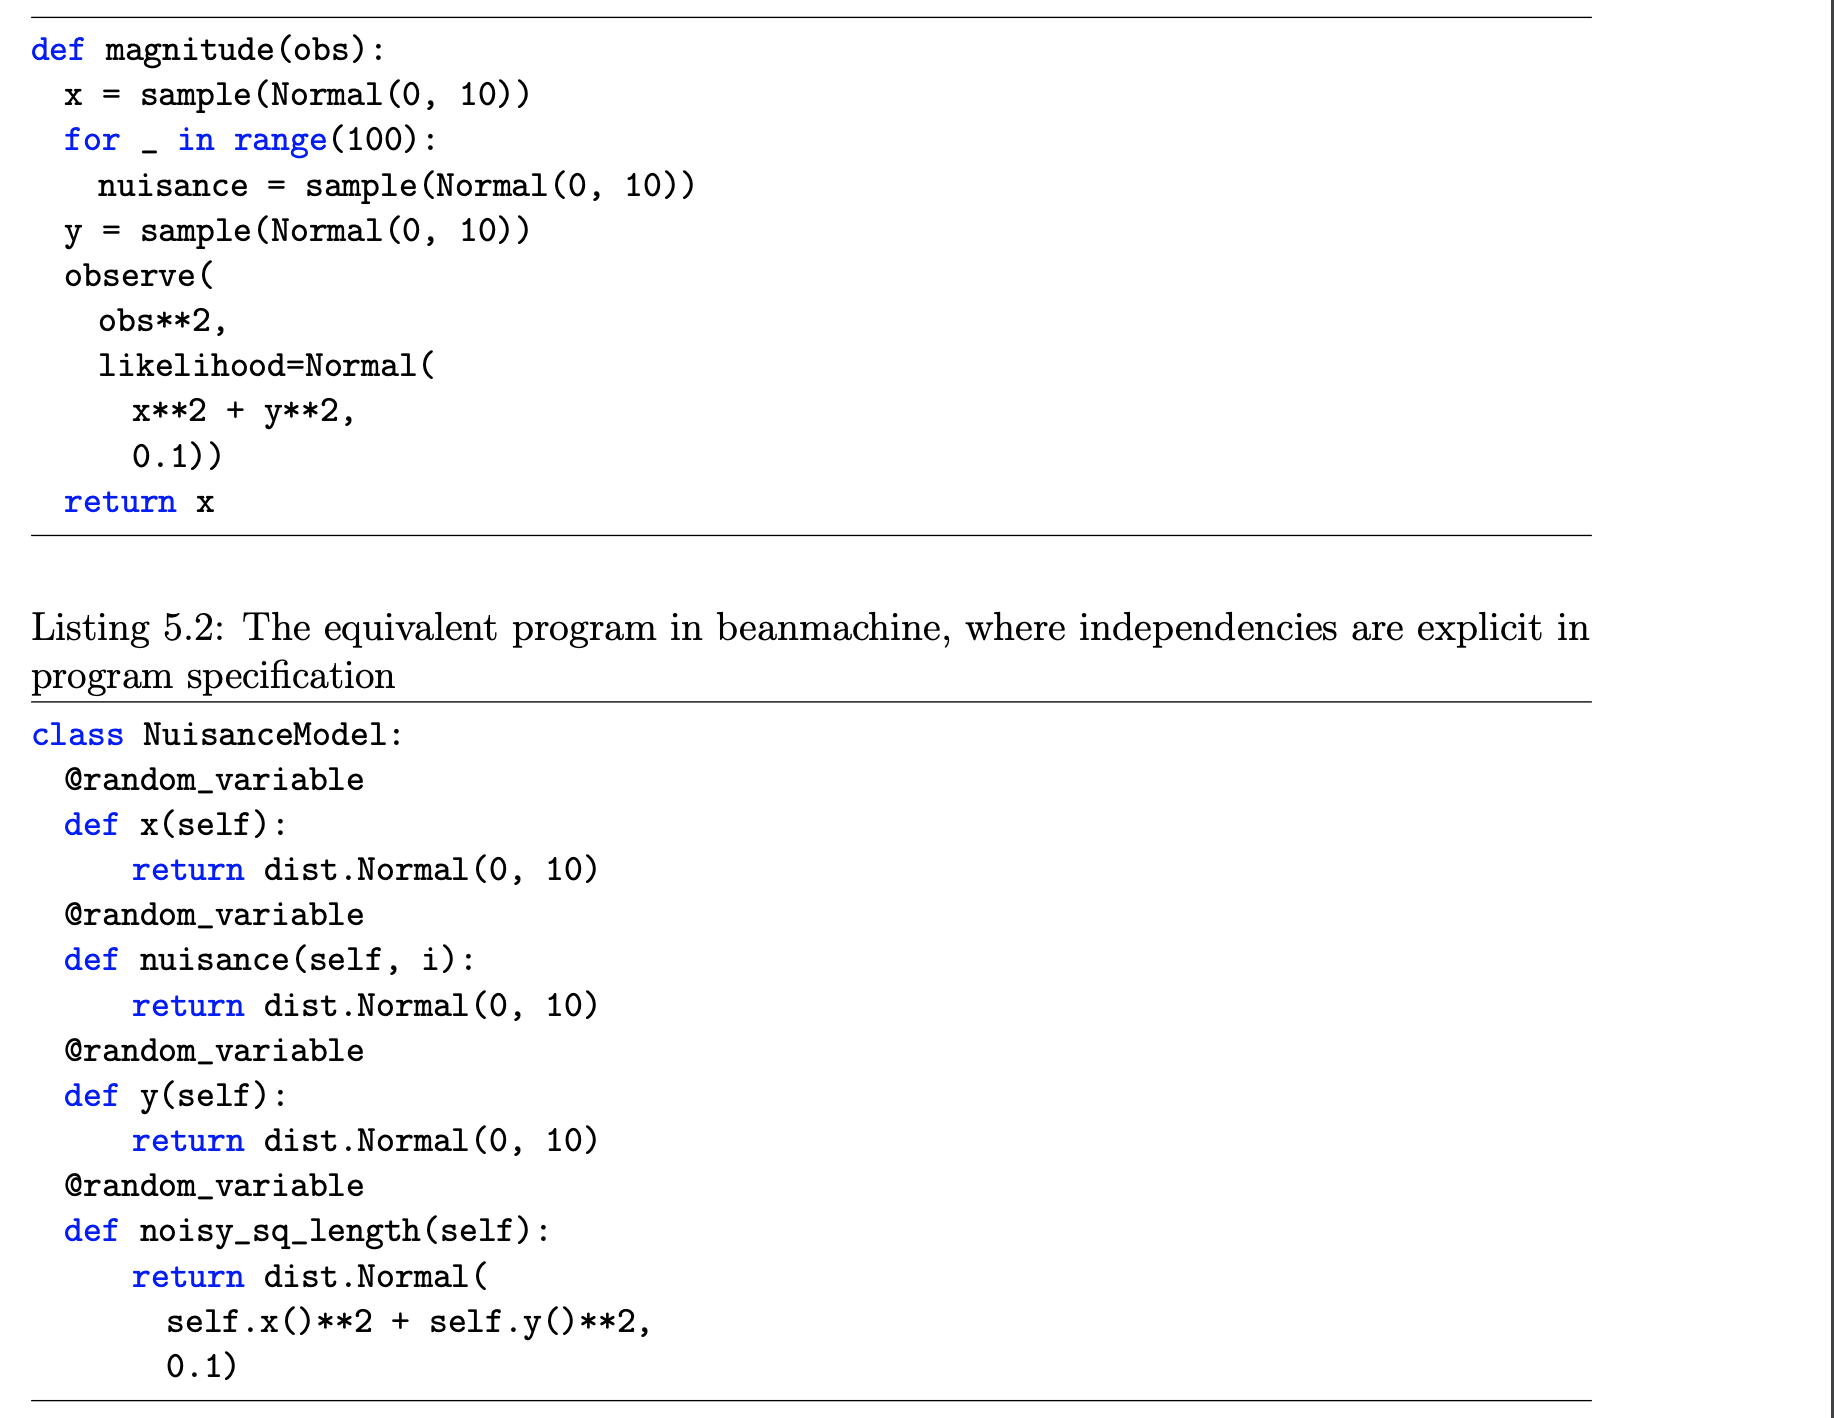
\includegraphics[width=0.4\textwidth,trim={0 0.5cm 20cm 12.5cm},clip]{Figures/lic/nuisance-progs.png}
    \end{figure}
    \begin{figure}
        \centering
        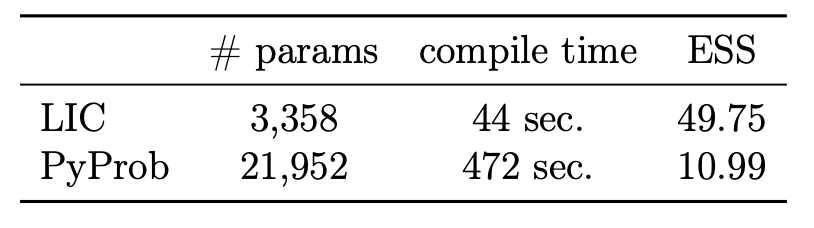
\includegraphics[width=0.6\textwidth]{Figures/lic/nuisance-params.png}
    \end{figure}
\end{frame}

\begin{frame}{Results: n-schools}
    \begin{figure}
        \centering
        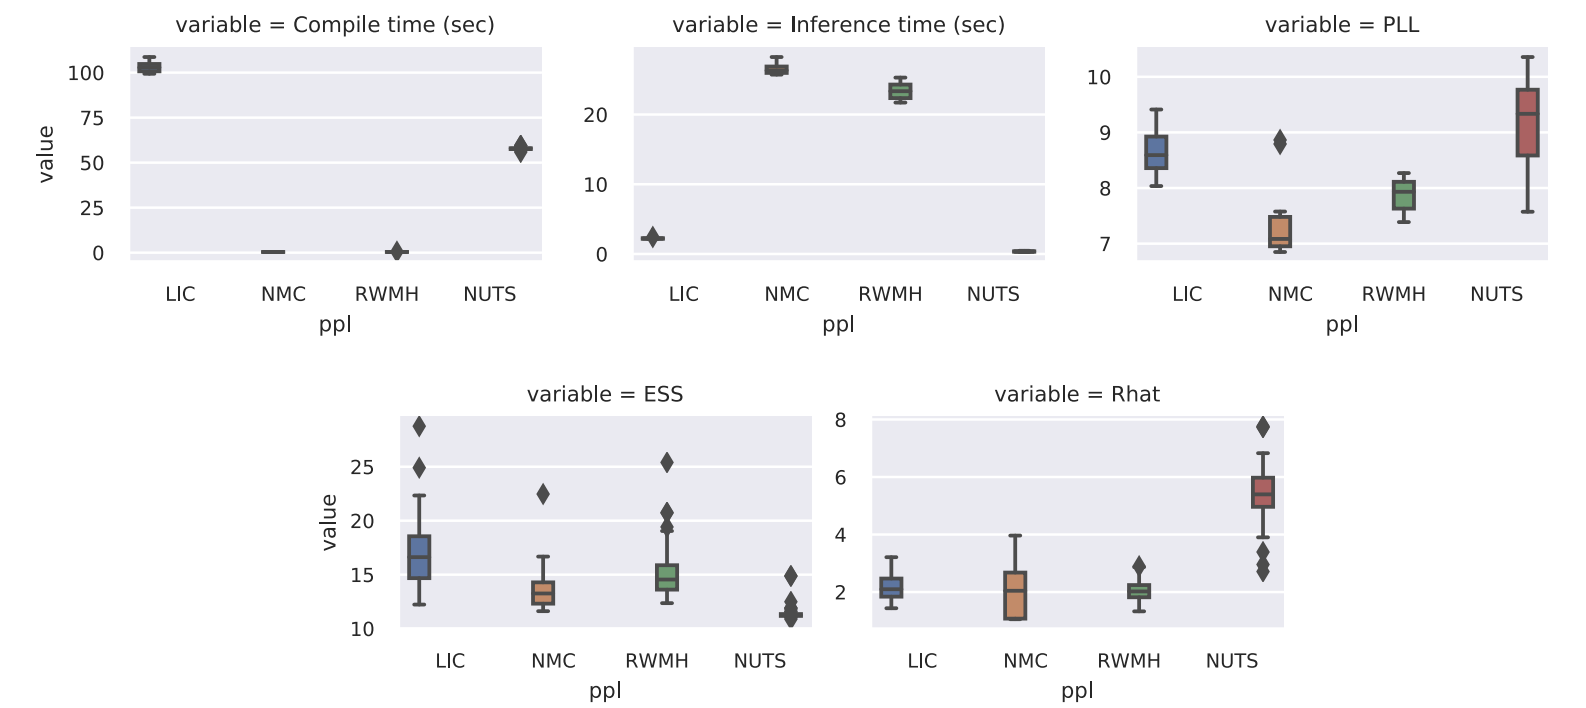
\includegraphics[width=\textwidth]{Figures/lic/nschools.png}
    \end{figure}
\end{frame}

\begin{frame}{Results: Bayesian logistic regression}
    \begin{figure}
        \centering
        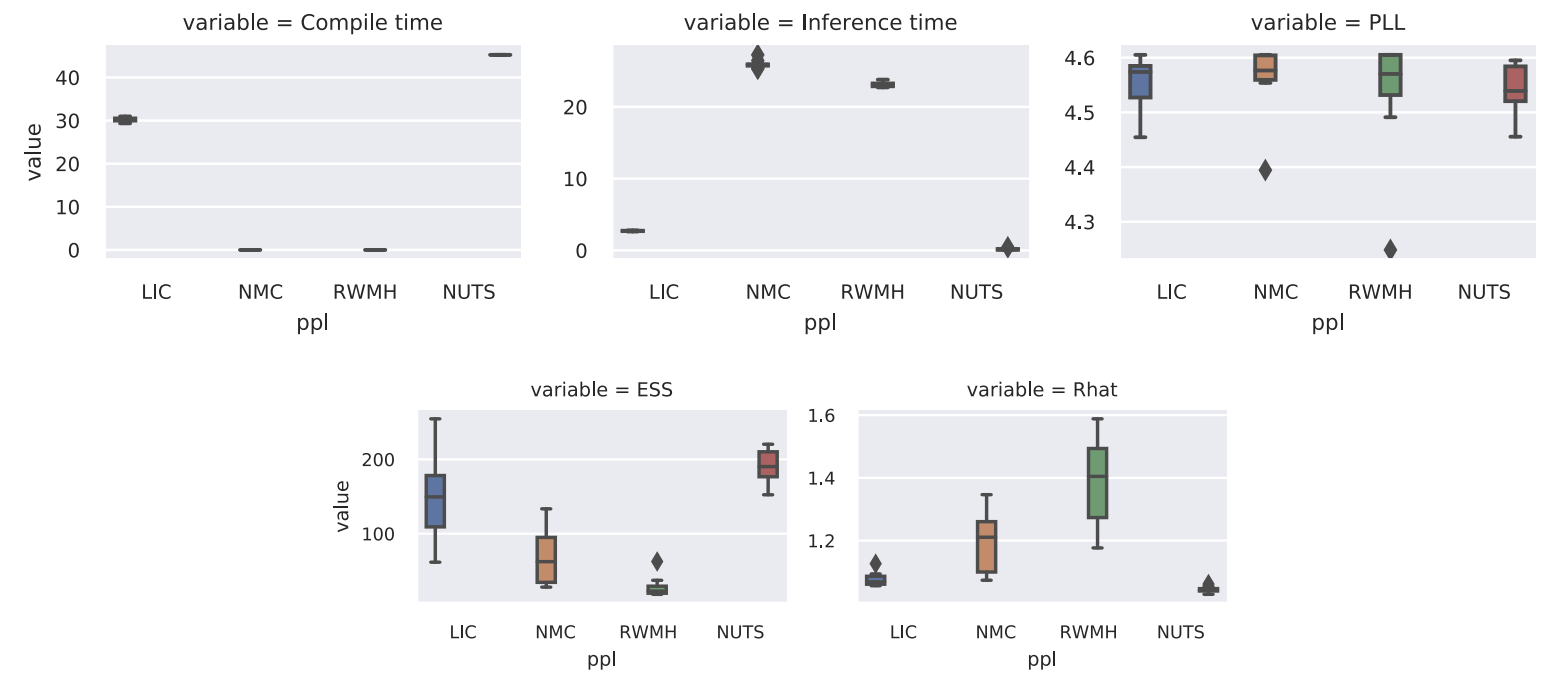
\includegraphics[width=\textwidth]{Figures/lic/blr.png}
    \end{figure}
\end{frame}

% \begin{frame}[fragile]{Normal-normal model}
% 	$p \sim N(0.0, 2.0)$, $x \sim N(p, 0.1)$,
	
% 	\textbf{Goal}: Draw samples $\Pr[p \mid x]$
	
% 	\textbf{Conjugacy}: Calculus shows $\Pr[p \mid x] = N(0.9975 x, 0.009975)$,
% 	member of variational family $\implies$ zero approximation error
	
% 	\note[itemize]{
% 	    \item Conjugate model where we know exact result is a precision weighted average
% 	    \item Posterior is normal, in variational family, no approximation error
% 	}
% \end{frame}

% \begin{frame}[fragile]{Random walk MH on Normal-Normal model}
%     \begin{figure}
%         \centering
%         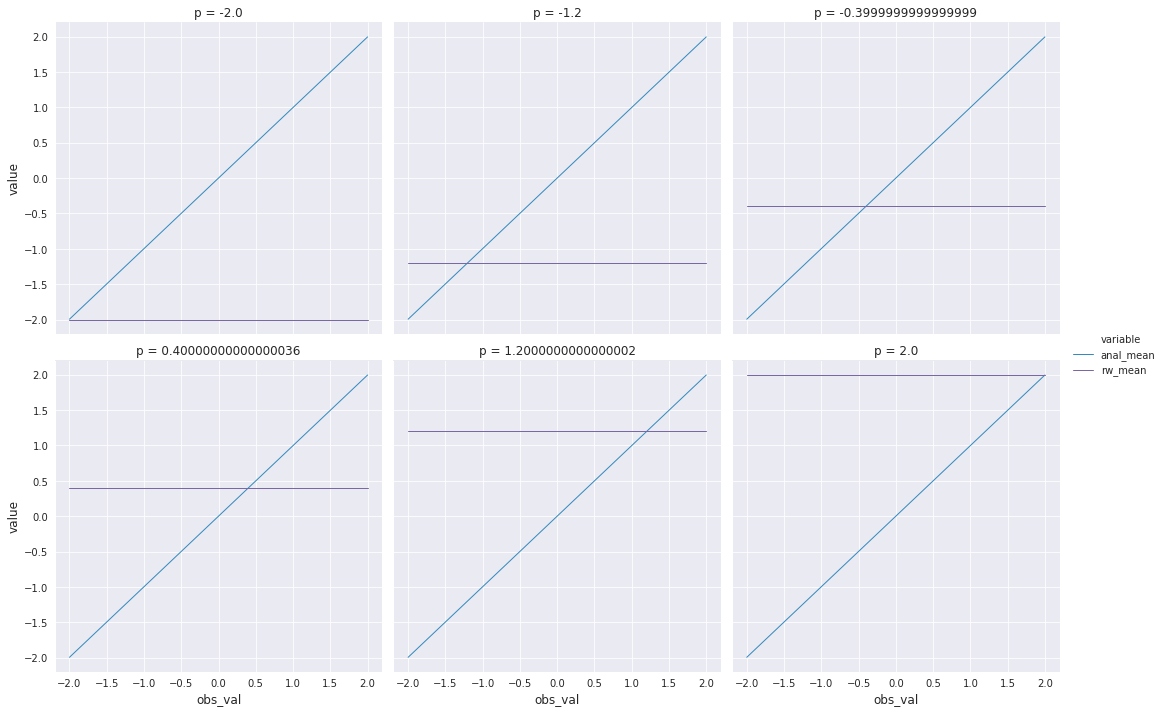
\includegraphics[width=\linewidth]{Figures/lic/rwmh.png}
%         \caption{Random walk MH's proposer mean depends on current value of $p$ in Markov chain}
%     \end{figure}
% \end{frame}

% \begin{frame}[fragile]{IC on Normal-Normal model: the good parts}
%     \begin{figure}
%         \centering
%         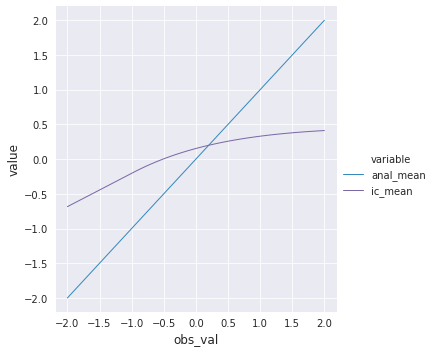
\includegraphics[width=0.7\linewidth]{Figures/lic/ic_normal_normal.png}
%         \caption{IC on Normal-Normal successfully captures posterior mean [n313855]}
%     \end{figure}
%     \note[itemize]{
%     \item Does not depend on current value of $p$
%     }
% \end{frame}

% \begin{frame}[fragile]{IC on Normal-Normal model: the bad parts}
%     Sensitive to initialization
%     \begin{figure}
%         \centering
%         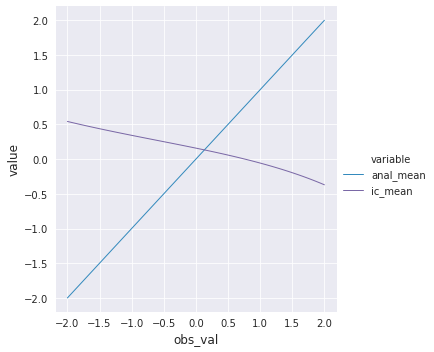
\includegraphics[width=0.48\linewidth]{Figures/lic/ic_normal_normal_fail_mean.png}
%         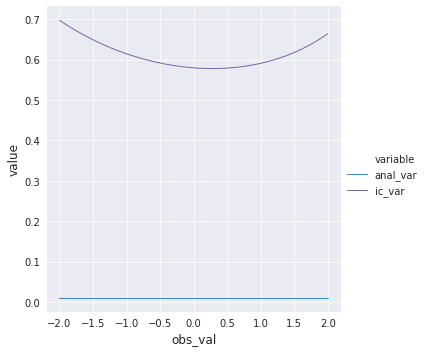
\includegraphics[width=0.48\linewidth]{Figures/lic/ic_normal_normal_fail_var.png}
%         \caption{Exploding variance on bad initializations [n313855]}
%     \end{figure}
%     \note[itemize]{
%         \item Depends on initialization, sometimes optimization explodes variance to maximize probability
%         \item NOTE: bad variational approximation could still give decent MCMC results; proposer covers support of posterior
%     }
% \end{frame}

% \begin{frame}[fragile]{IC on Normal-Normal model: the bad parts}
%     Local optima problems mitigated by reducing model parameters
%     \begin{figure}
%         \centering
%         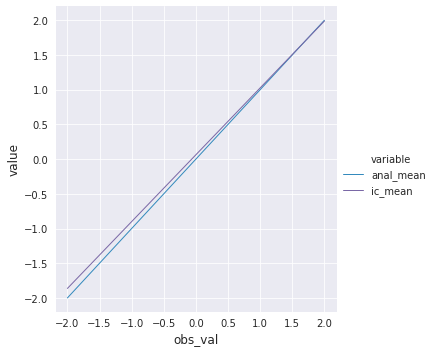
\includegraphics[width=0.6\linewidth]{Figures/lic/ic_normal_normal_linear.png}
%         \caption{IC with appropriate model size accurately captures posterior mean [n313855]}
%     \end{figure}
%     \note[itemize]{
%         \item 1D observation embedding, no activation functions => can only learn linear functions
%         \item Works here, but not general. Will look at regularization to reduce hypothesis space later.
%     }
% \end{frame}


% \begin{frame}[fragile]{Vectorized n-schools}
% 	\begin{figure}
% 	    \centering
% 	    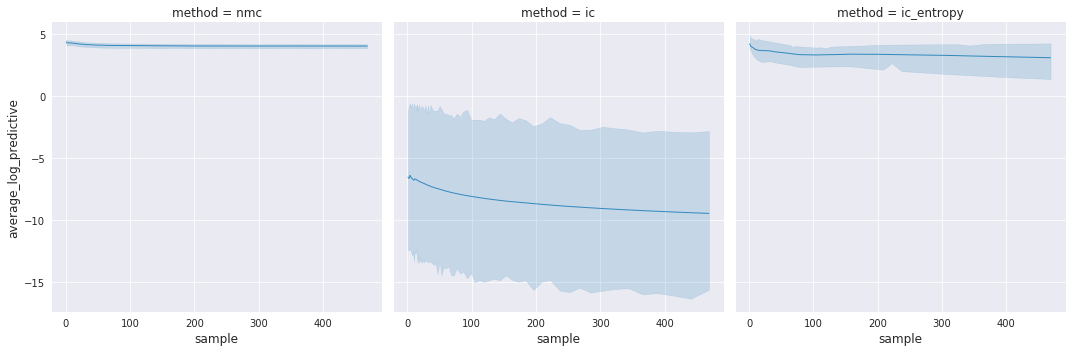
\includegraphics[width=0.9\linewidth]{Figures/lic/nschools-pll.png}
% 	    \caption{Predictive log likelihoods on vectorized n-schools [D22448718]}
% 	\end{figure}
% \end{frame}

% \begin{frame}[fragile]{Vectorized n-schools}
% 	\begin{figure}
% 	    \centering
% 	    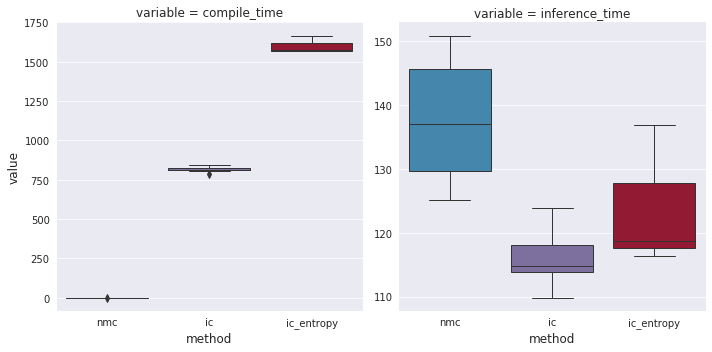
\includegraphics[width=0.7\linewidth]{Figures/lic/nschools-compile-infer-time.png}
% 	    \caption{IC amortizes compilation costs (10,000 worlds above) through faster inference runtimes}
% 	\end{figure}
% \end{frame}

% \begin{frame}[fragile]{Vectorized n-schools}
% 	\begin{figure}
% 	    \centering
% 	    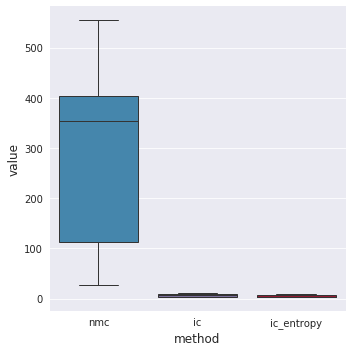
\includegraphics[width=0.4\linewidth]{Figures/lic/nschools-ic-neff.png}
% 	    \caption{IC yields very low ESS (no burn in, 500 samples)}
% 	\end{figure}
% \end{frame}

% \subsection{Limitations and next steps}

% \begin{frame}[fragile]{Limitations and next steps}
%     \begin{itemize}
%         \item Other variational families (eg GMM, IAF)
%         \item Entropy regularization to address exploding variance
%         \begin{align*}
%             \mathcal{L}(\phi)
%             &= D_{KL}(p(\vec{x} \mid \vec{y}) || q(\vec{x} \mid \vec{y}; \phi) ) + H(q(\vec{x} \mid \vec{y}; \phi))
%         \end{align*}
%     \end{itemize}
    
%     \begin{figure}
%         \centering
%         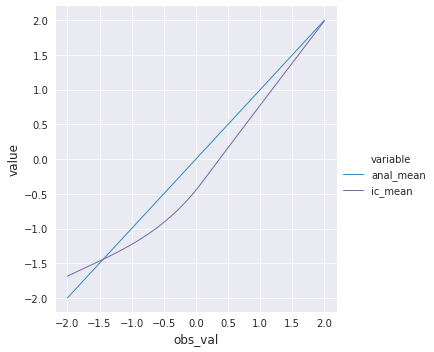
\includegraphics[width=0.4\linewidth]{Figures/lic/ic-entropy-mean.png}
%         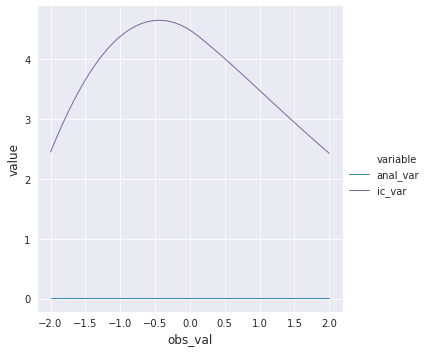
\includegraphics[width=0.4\linewidth]{Figures/lic/ic-entropy-var.png}
%         \caption{Entropy regularization penalizes exploding variance, favoring a better variational approximation in Normal-Normal
%         [n313855]}
%     \end{figure}

% 	\note[itemize]{
% 	    \item Currently only diagonal normal (mean-field) and categorical variational families, GMM and IAF can both capture multimodal densities as well as correlations
% 	    \item Entropy regularization penalizes exploding variance; how to theoretically justify?
% 	}
% \end{frame}


% \appendix


% \begin{frame}[fragile]{Contribution: Online Adaptation}
%     \textbf{Problem}: forward samples during compilation may not sufficiently represent observations ($\text{obs}$) encountered at inference
    
%     \textbf{Solution}: perform MCMC with IC artifact to draw posterior samples $(\vec{x}^{(m)}, \vec{y}^{(m)}=\text{obs}) \sim P(\vec{x} \mid \vec{y}=\text{obs})$,
%     hill-climb inclusive KL between \emph{conditional} (rather than joint) posterior
%     \begin{align*}
%         &\argmin_{\phi} D_{KL}(p(\vec{x} | \vec{y}=\text{obs}) || q(\vec{x} | \vec{y}=\text{obs}; \phi)) \\
%         &\approx 
%         \argmin_{\phi} \sum_{m=1}^N \log Q(\vec{x}^{(m)} \mid \vec{y} = \text{obs}, \phi)
%     \end{align*}
% \end{frame}


% \begin{frame}[fragile]{IC on Normal-Normal model: the bad parts}
%     Also affects \cite{le2017inference}
%     \begin{figure}
%         \centering
%         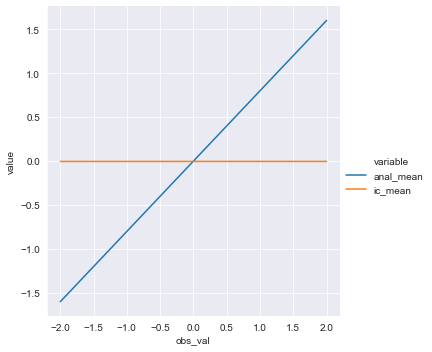
\includegraphics[width=0.48\textwidth]{Figures/lic/ic-smc-fail.png}
%         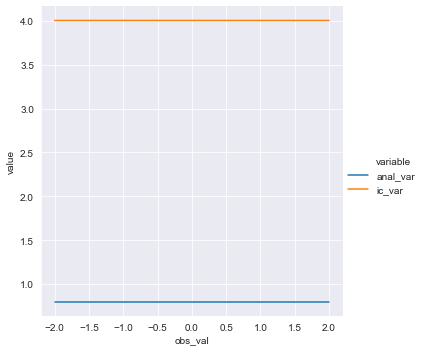
\includegraphics[width=0.48\textwidth]{Figures/lic/ic-smc-fail-var.png}
%         \caption{\texttt{pyprob}'s\footnote{\tiny\url{https://github.com/pyprob/pyprob/}} IC also exhibits variance explosion
%         \footnote{\tiny\url{https://github.com/facebookexternal/ppl_papers/blob/master/ic/Normal-Normal\%20convergence\%20studies.ipynb
%         }}}
%     \end{figure}
% \end{frame}

% \section{Bayesian Experimental Design}

\begin{frame}
  \frametitle{Bayesian experimental design}
  Consider $n$ parameterized experiments:
  $\x_1,\dots,\x_n\in\R^d$.\\
  Each experiment has a real random response $y_i$ such that:
  \begin{align*}
    y_i = \x_i^\top\w^* + \xi_i,\qquad \xi_i\sim\Nc(0,\sigma^2),\quad \Blue{\w^*\sim\Nc(0,\sigma^2\A^{-1})}
  \end{align*}
\textbf{Goal:} Select $k\ll n$ experiments to best estimate $\w^*$
\pause
\begin{columns}
\begin{column}{0.3\textwidth}
\\ \vspace{0.8cm}
Select $S=\{4,6,9\}$\\
\vspace{1cm}
Receive $y_4, y_6, y_9$
\end{column}
\begin{column}{0.5\textwidth}
\begin{center}
	\begin{tikzpicture}[scale=0.9]
          \draw [fill=brown!30] (-2,0) rectangle (0,3);
          \draw [color=black] (-2,2) -- (0,2);
          \draw (-2.25,2) node {\mbox{\footnotesize $\x_4^\top$}}; 
          \draw [color=black] (-2,1.5) -- (0,1.5);
          \draw (-2.25,1.5) node {\mbox{\footnotesize $\x_6^\top$}}; 
          \draw [color=black] (-2,0.5) -- (0,0.5);
          \draw (-2.25,0.5) node {\mbox{\footnotesize $\x_9^\top$}}; 
	   \draw (-2.8,3) node {\footnotesize fixed $\X$}; 
          \draw [decorate,decoration={brace}] (-2,3.1) -- (0,3.1);
          \draw (-1,3.4) node {\mbox{\fontsize{8}{8}\selectfont $d$}}; 
            \draw [color=lightgray,line width =0.5mm] (1,0) -- (1,3);
            \draw [color=lightgray] (0.75,3) node {$\y$};
            \draw (0.75,2) node {\mbox{\footnotesize $y_4$}}; 
            \draw (1,2) node {.}; 
            \draw[mark=*,mark size=1.5pt] plot coordinates{(1,2)};
            \draw (0.75,1.5) node {\mbox{\footnotesize $y_6$}}; 
            \draw (1,1.5) node {.}; 
            \draw[mark=*,mark size=1.5pt] plot coordinates{(1,1.5)};
            \draw (0.75,0.5) node {\mbox{\footnotesize $y_9$}}; 
            \draw[mark=*,mark size=1.5pt] plot coordinates{(1,.5)};
	\end{tikzpicture}
\end{center}
\end{column}
\end{columns}
\end{frame}

\begin{frame}
  \frametitle{Bayesian A-optimal design}
Given the Bayesian assumptions, we have
  \begin{align*}
  \w\mid \y_S \ \sim\ \Nc\Big(\ (\X_S^\top\X_S + \A)^{-1}\X_S^\top\y_S
  ,\ \ \sigma^2(\X_S^\top\X_S+\A)^{-1}\ \Big),
  \end{align*}
  
  Bayesian A-optimality criterion:
\begin{align*}
f_{\A}(\X_S^\top\X_S)=\tr\big((\X_S^\top\X_S+\A)^{-1}\big).
\end{align*}

\textbf{Goal:} Efficiently find subset $S$ of size $k$ such that:
\begin{align*}
f_{\A}(\X_S^\top\X_S)\leq (1+\epsilon)\cdot\underbrace{\min_{S':|S'|=k}f_{\A}(\X_{S'}^\top\X_{S'})}_{\opt}
\end{align*}
\end{frame}

\begin{frame}
  \frametitle{Relaxation to a semi-definite program}
  \begin{block}{SDP relaxation}
The following can be found via an SDP solver in polynomial time:
  \begin{align*}
p^* \ = \  \argmin_{p_1,...,p_n}\ \
  f_{\A}\Big(\sum_{i=1}^np_i\x_i\x_i^\top\Big),\\
\text{subject to}\quad
  \forall_i\ \ 0\leq p_i\leq 1,\quad \sum_i p_i=k.
  \end{align*}
\end{block}

\pause

The solution $p^*$ satisfies $f_{\A}\big(\sum_{i}p_i \x_i \x_i^\top\big)\leq\opt$.

\pause

\textbf{Question:}
For what $k$ can we efficiently round this to $S$ of size $k$?
    
\end{frame}

\begin{frame}
  \frametitle{Efficient rounding for \emph{effective dimension} many
    points\footnote{\tiny\fullcite{bayesian-experimental-design}}}
  \begin{definition}
Define $\A$-effective dimension as $d_{\A} =\tr\big(\X^\top\X(\X^\top\X+\A)^{-1}\big) \leq d$.
\end{definition}
\pause
  \begin{theorem}
If $k=\Omega\big(\frac{d_{\A}}{\epsilon} +
\frac{\log1/\epsilon}{\epsilon^2}\big)$,
then there is a polynomial time 
  algorithm that finds subset $S$ of size $k$ such that
  \begin{align*}
    f_{\A}\big(\X_S^\top\X_S\big) \leq (1+\epsilon)\cdot\opt.
  \end{align*}
\end{theorem}

\pause

\textbf{Remark:} Extends to other Bayesian criteria:
C/D/V-optimality.

\pause

\textbf{Key idea:} \ Sampling $k$-DPP that depends on SDP solution and $\A$

\vspace{5mm}
\end{frame}

\begin{frame}
  \frametitle{Comparison with prior work}
  \centering
    \renewcommand{\arraystretch}{1.5}
\begin{tabular}{r||c|c|l}
 &Criteria&Bayesian&$k=\Omega(\cdot)$\\
  \hline\hline
\small (WYS17) %\cite{tractable-experimental-design}
  &\small A,V&\xmark&$\frac{d^2}{\epsilon}$\\
\small (ALSW17) %\cite{near-optimal-design}
  &\small A,C,D,E,G,V&\cmark&$\frac {d}{\epsilon^2}$\\
\small (NST19) %\cite{proportional-volume-sampling}
  &\small A,D&\xmark&$\frac{d}{\epsilon} +
  \frac{\log1/\epsilon}{\epsilon^2}$\\
  \hline
\small\textbf{our result} (DLM20)%\cite{bayesian-experimental-design}
&\small A,C,D,V&\cmark& $\frac{d_{\A}}{\epsilon} +
  \frac{\log1/\epsilon}{\epsilon^2}$
\end{tabular}
\end{frame}

\begin{frame}{Experiments}
    \begin{figure}
        \centering
        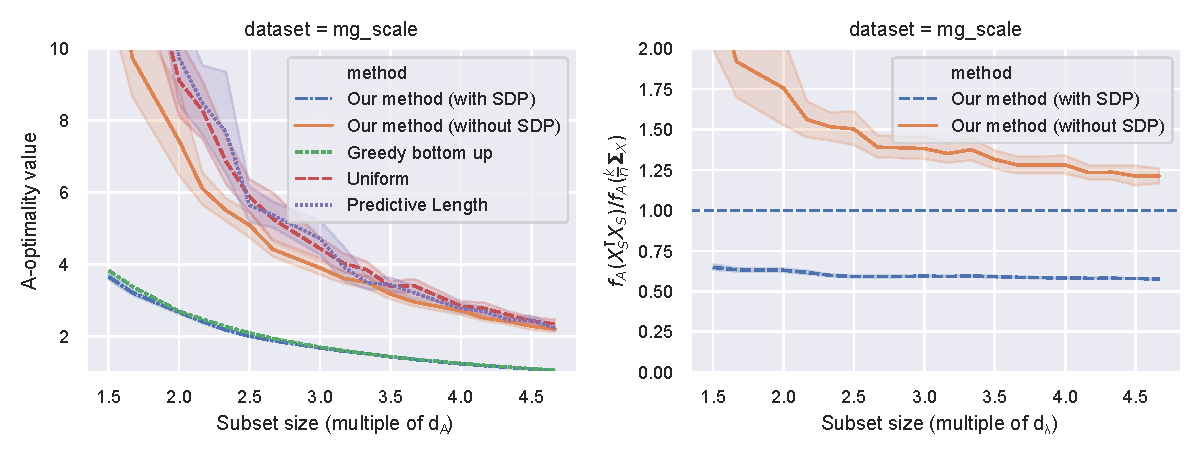
\includegraphics[width=\textwidth]{Figures/design/mg_combined.pdf}
    \end{figure}
\end{frame}

% \section{Double Descent}

% \begin{frame}
%   \frametitle{Supervised learning}
% Input:\hspace{1.95cm} $\x\sim \mu$,\\
% Label:\hspace{1.9cm} $y = f^*(\x) + \xi$,\hspace{2cm}$\xi$ - noise\\[5mm]
%   \pause
%   Training data:\hspace{.5cm} $(\x_1,y_1),...,(\x_n,y_n)$ \\[5mm]
%   \pause
% \model
% \pause      \vspace{5mm}
      
% Error:\hspace{1.9cm} $\MSE{f_\w}=\E\,\|f_\w-f^*\|^2$
        
% \end{frame}

\begin{frame}
  \frametitle{When do supervised models learn?}
  
  Goal: $\MSE{f_\w} \ll \MSE{f_{\mathrm{null}}}$,  $f_{\mathrm{null}}\equiv 0$

\pause
  
``Classical'' answer (e.g., VC theory): use $n \gg d$
  \begin{quote}
    Models learn when there is more \emph{data} than \emph{parameters}.
  \end{quote}
  
  \vspace{5mm}

  
``Modern'' answer (e.g., deep learning): use $d \gg n$
  \begin{quote}
    Models learn when there is more \emph{parameters} than \emph{data}.
  \end{quote}

  \vspace{5mm}

  How to reconcile the two paradigms?
\end{frame}

\begin{frame}
  \frametitle{Simple model: linear regression}
  \begin{columns}
    \begin{column}{0.5\textwidth}
      \vspace{2mm}
      
      Standard i.i.d.~random design\\
$\X\sim\mu^n$\\
$\y=\X\w+\xib$\qquad$\xib\sim\Nc(\vec{0},\sigma^2\I)$
    \end{column}
    \begin{column}{0.4\textwidth}
      \begin{tikzpicture}[scale=0.9]
        \draw [fill=brown!30] (-2,1.5) rectangle (0,3);
        \draw [color=black] (-2,2) -- (0,2);
        \draw (-1,2.2) node {\mbox{\footnotesize $\x_i^\top$}}; 
        \draw (-2.5,3) node {$\X$}; 
        \draw [decorate,decoration={brace}] (-2,3.1) -- (0,3.1);
        \draw (-1,3.4) node {\mbox{\fontsize{8}{8}\selectfont $d$}}; 
        \draw [decorate,decoration={brace}] (-2.1,1.5) -- (-2.1,3);
        \draw (-2.4,2.25) node {\mbox{\fontsize{8}{8}\selectfont $n$}}; 
        \draw [color=black,line width =0.5mm] (1,1.5) -- (1,3);
        \draw [color=black] (0.75,3) node {$\y$};
      \end{tikzpicture}
    \end{column}
  \end{columns}
  
  \pause
  
  Goal:\quad find\quad$\MSE{\X^\dagger\y}=\E\,\|\X^\dagger\y-\w\|^2$ where
  the
  Moore-Penrose estimator:
  \begin{align*}
    \X^\dagger\y =
      \begin{cases}
        \text{minimum norm solution},& \text{for }n\leq d,\\
        \text{least squares solution},& \text{for }n>d.
      \end{cases}
  \end{align*}
  
  \pause

    Prior work: asymptotics \cite{HMRT19_TR} and upper bounds
    \cite{BLLT19_TR}
    
  \textcolor{red}{No closed form expressions, even for
    $\mu=\Nc(\vec{0},\Sigmab)$!}
\end{frame}

\begin{frame}
  \frametitle{Main result I: exact non-asymptotic MSE}
  Idea: replace standard i.i.d.~design with a surrogate design
  \begin{align*}
    \underbrace{\X\sim\mu^n}_{\text{i.i.d.}}\qquad\Longrightarrow\qquad
    \underbrace{\Xb\sim S_\mu^n}_{\text{surrogate}} 
  \end{align*}
  \pause\vspace{-2mm}
  \begin{theorem}
\label{t:mse}
Let \ $\Xb\sim S_\mu^n$, \ $\yb_i=\xbb_i^\top\w+\xi$ \ and \
$\Sigmab_\mu=\E_\mu[\x\x^\top]$. Then,
  \begin{align*}
 &\MSE{\Xb^\dagger\ybb} =\\
  &  \begin{cases}
    \sigma^2\,\tr\big((\Sigmab_\mu+\lambda_n\I)^{-1}\big)
    \frac{1-\alpha_n}{d-n}\ +\
\frac{\w^{\top}(\Sigmab_\mu+\lambda_n\I)^{-1}\w}
{\tr((\Sigmab_\mu+\lambda_n\I)^{-1})}(d-n),
& (n<d),\\
\sigma^2\, \tr(\Sigmab_\mu^{-1}),& (n=d),\\
\sigma^2\,\tr(\Sigmab_\mu^{-1})\frac{1-\beta_n}{n-d},&(n>d),
\end{cases}
  \end{align*}
  \pause where
  $n=\tr((\Sigmab_\mu+\lambda_n\I)^{-1}\Sigmab_\mu)$, \
  $\alpha_n=\frac{\det(\Sigmab_\mu)}{\det(\Sigmab_\mu+\lambda_n\I)}$,
\ $\beta_n=\ee^{d-n}$.
\end{theorem}
\end{frame}

\begin{frame}
  \frametitle{Isotropic features: double descent curve}
  $\X\sim\mu^n$ \ - standard Gaussian design, $\mu=\Nc(\vec{0},\I)$, $d=100$

      \begin{align*}
        \MSE{\X^\dagger\y} =
        \begin{cases}
          \frac{\sigma^2n}{d-n-1} + \|\w\|^2\frac{d-n}{d},&(n<d-1)\\
          \frac{\sigma^2d}{n-d-1},&(n>d+1)
        \end{cases}\quad(\text{let }\|\w\|=1)
      \end{align*}
      \vspace{-2mm}
      \begin{figure}
          \centering
          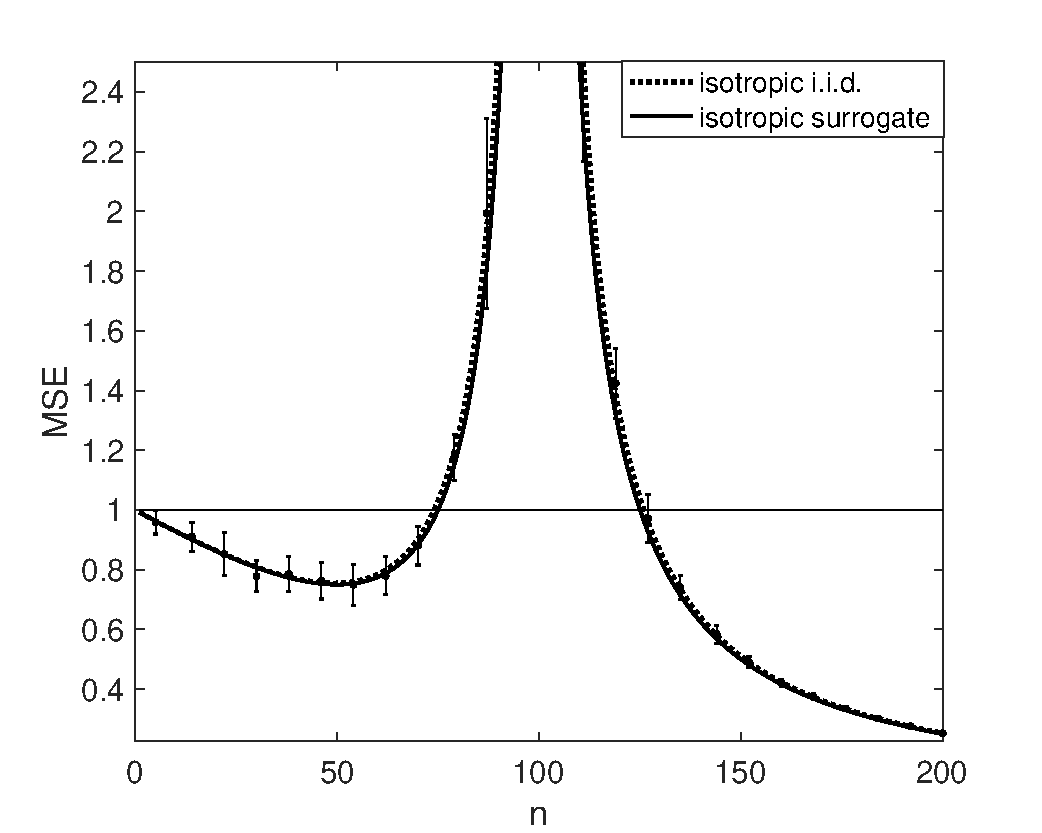
\includegraphics[width=0.7\textwidth]{Figures/descent/descent-isotropic.pdf}
      \end{figure}
\end{frame}

\begin{subframe}
  \frametitle{Gaussian features: effect of spectral decay}
  $\X\sim\mu^n$ \ - multivariate Gaussian design,
  $\mu=\Nc(\vec{0},\Sigmab)$, $d=100$\\
$\Sigmab$ \ - exponentially decaying eigenvalues, condition
number $\kappa$
\pause
\begin{align*}
\MSE{\X^\dagger\y}\ =\ ?
  \end{align*}
  \pause \vspace{-3mm}
  \begin{figure}
      \centering
      \includegraphics[width=0.7\textwidth]{Figures/descent/descent-full}
  \end{figure}
\end{subframe}

\begin{subframe}
  \frametitle{Gaussian features: effect of model complexity}
    $\X\sim\mu^n$ \ - multivariate Gaussian design,
  $\mu=\Nc(\vec{0},\Sigmab)$, $n=100$\\
$\Sigmab$ \ - exponentially decaying eigenvalues, condition
number $\kappa$
\begin{align*}
\MSE{\X^\dagger\y}\ =\ ?
  \end{align*}\vspace{-3mm}
  \begin{figure}
      \centering
    \includegraphics[width=0.7\textwidth]{Figures/descent/descent-model}
  \end{figure}
\end{subframe}

\begin{frame}
  \frametitle{Main result II: implicit regularization of minimum norm}
Why does this \textit{unregularized} model learn when $n<d$?\\
  \pause
\textit{Because taking minimum norm induces
  $\ell_2$-regularization.}
\vspace{2mm}
\pause
\begin{theorem}
Let \ $\Xb\sim S_\mu^n$, \ $\yb_i=y(\x)$ \ and \
$\Sigmab_\mu=\E_\mu[\x\x^\top]$. Then,
 \begin{align*}
    \E\big[\Xb^\dagger\ybb\big] = 
    \begin{cases}
      (\Sigmab_\mu + \lambda_n\I)^{-1}\v_{\mu,y} &\text{for }n<d,\\
        \Sigmab_\mu^{-1}\v_{\mu,y} &\text{for }n \ge d,
    \end{cases}
 \end{align*}
  where \ $n=\tr((\Sigmab_\mu+\lambda_n\I)^{-1}\Sigmab_\mu)$ \ and \ $\v_{\mu,y}=\E_\mu[y(\x)\,\x ]$.
\end{theorem}
\pause
\begin{align*}
  (\Sigmab_{\mu} +  \lambda_{n}\I)^{-1} \v_{\mu,y}
  \ =\ \argmin_{\wbh} \ \E_{\mu,y}\Big[\big(\x^\top\wbh-y(\x)\big)^2\Big]
    + \lambda_n\|\wbh\|^2
\end{align*}
\end{frame}

\begin{subframe}
  \frametitle{Implicit regularization}
  Our observations:\\
  \begin{itemize}
    \item Minimum norm induces an $\ell_2$-regularizer:
      $\lambda_n\|\wbh\|^2$\pause
\item Sample size is effective dimension:
  $n=\tr((\Sigmab_\mu+\lambda_n\I)^{-1}\Sigmab_\mu)$
  \end{itemize}\pause
%\vspace{5mm}

~\hspace{-0.8cm}\includegraphics[width=0.57\textwidth]{Figures/descent/descent-bias}\nobreak\includegraphics[width=0.57\textwidth]{Figures/descent/descent-lambda}
\end{subframe}

\begin{frame}
  \frametitle{Asymptotic consistency of surrogate expressions}
  \begin{align*}
  \MSE{\X^\dagger\y}
  &=\sigma^2\E\big[\tr\big((\X^\top\X)^\dagger\big)\big] +
    \w^{\top}\E\big[\I-\X^\dagger\X\big]\w.
  \end{align*}
  \begin{align*}
    \mu=\Nc(\vec{0},\Sigmab)\quad \Longrightarrow\quad
    \begin{cases}
      \X^\top\X&-\quad\text{Wishart distribution}\\
      \X^\dagger\X&-\quad\text{Gaussian projection}
    \end{cases}
  \end{align*}
  \pause
  \begin{conjecture}
  Fix $n/d<1$ and let $\mu=\Nc(\vec{0},\Sigmab )$, where 
  $c\I\preceq\Sigmab\preceq C\I$. Then:
\begin{align*}
\bigg|\frac{\E\big[\tr((\X^\top\X)^\dagger)\big]}{\Vc(\Sigmab,n)} -1\bigg|&=
  O(1/d)\quad\text{for}\quad\Vc(\Sigmab,n)=\frac{1-\alpha_n}{\lambda_n},\\
%\sup_{\w\in\R^d}
  \bigg|\frac{\w^\top\E[\I-\X^\dagger\X]\w}{\w^\top
  \Bc(\Sigmab,n)\w} - 1\bigg| &= O(1/d)\quad\text{for}\quad
  \Bc(\Sigmab,n) = \lambda_n(\Sigmab+\lambda_n\I)^{-1}
\end{align*}
\end{conjecture}
\end{frame}

\begin{frame}
  \frametitle{Empirical evidence for the conjecture}
~\hspace{-1cm}\includegraphics[width=1.16\textwidth]{Figures/descent/wishart_var.pdf}\\
~\hspace{-1cm}\includegraphics[width=1.16\textwidth]{Figures/descent/proj_bias.pdf}
\end{frame}

\begin{subframe}
  \frametitle{Surrogate design: rescaling by pseudo-determinant}
  \begin{definition}
    Let $K$ be a random variable over non-negative integers. \\
    A determinantal surrogate design
    $\Xb\sim \Det(\mu,K)$ is defined so that
\begin{align*}
  \E\big[F(\Xb)\big]\  \propto\ \E[\pdet(\X\X^\top)F(\X)]
  \quad\text{for}\quad\X\sim\mu^K.
\end{align*}
\end{definition}
\begin{itemize}
  \pause
\item The proportionality constant is $1/\E[\pdet(\X\X^\top)]$.
\pause
\item To compute it, we let $K$ be a Poisson random variable.
\pause
\item New expectation formulas for $K\sim\Poisson(\gamma)$ and $\X\sim\mu^K$:
\begin{align*}
  \E\big[\det(\X\X^\top)\big]
  &= \ee^{-\gamma}\det(\I+\gamma\Sigmab_\mu)\\
  \E\big[\det(\X^\top\X)\big]
  &= \det(\gamma\Sigmab_\mu)
\end{align*}
\end{itemize}

\end{subframe}

\begin{subframe}
  \frametitle{New technique: \textit{determinant preserving random
      matrices}}
\begin{definition}
A random $d\times d$ matrix $\A$ is \emph{determinant
  preserving} (d.p.) if
\begin{align*}
  \E\big[\!\det(\A_{\Ic,\Jc})\big] =
  \det\!\big(\E[\A_{\Ic,\Jc}]\big)\quad \text{for all }\Ic,\Jc\subseteq
  [d]\text{ s.t. }|\Ic|=|\Jc|.
\end{align*}
\vspace{-7mm}
\end{definition}
\pause
Examples:
  \begin{itemize}
  \item $\A$ has i.i.d.~Gaussian entries  $a_{ij}\sim\Nc(0,1)$\pause    
  \item $\A = s\Z$, where $s$ is random and $\Z$ is a fixed,
    rank-1 matrix\pause
    \item $\A=\X^\top\X$, where $\X\sim\mu^K$ and $K\sim\Poisson(\gamma)$
    \end{itemize}
    \pause
  \begin{theorem}[closure properties]
    If $\A,\B$ are d.p.~and independent, then $\A+\B$ and $\A\B$ are
    also d.p.
  \end{theorem}
\end{subframe}

% \section{Sub-Gaussian Projections}


\begin{frame}{Matrix sketching}

\begin{center}
  
  \begin{tikzpicture}[scale=1.0]
    \draw[fill=blue!20] (-4.5,3) rectangle (-0.5,4);
%        \draw (-1.5,2.5) node {$\S$};
%        \draw (0,2.5) node {$\times$};
    \draw[fill=blue!20] (0.5,0) rectangle (3,4);
    \draw[fill=blue!20] (4,3) rectangle (6.5,4);
    \draw (1.3,2.5) node {$\S \qquad\qquad\qquad\qquad \A \qquad\qquad\qquad\tilde\A$};
%        \draw (3.5,2.5) node{$=$};
    \draw (1,3.5) node {\mbox{
        sub-gaussian\qquad$\times$\qquad data \qquad$=$\qquad sketch}};
%        \draw (5,2.5) node {$\tilde\A$};
% \draw[fill=blue!20] (1,0) rectangle (2.5,4);
%    \draw (2,2) node {\mbox{$\A$}};
%    \draw (6.5,2) node {\mbox{$\in\R^{m\times n}$}};
  \end{tikzpicture}
\end{center}
Least squares, stochastic optimization, data compression,
approximate SVD
\end{frame}
    

\begin{frame}{Residual projection matrix}

\begin{center}      
    \begin{tikzpicture}[scale=1.0]

    \draw (-3.2,-3.2) -- (3.2,3.2);
    \tkzDefPoint(0,1){A};         \tkzDefPoint(0.5,.5){A1}; \tkzDrawSegment[thick,red](A,A1);
    \tkzDefPoint(1.8,.5){B};     \tkzDefPoint(1.15,1.15){B1}; \tkzDrawSegment[thick,red](B,B1);
    \tkzDefPoint(2.5,1.5){C};   \tkzDefPoint(2,2){C1}; \tkzDrawSegment[thick,red](C,C1);
    \tkzDefPoint(-1.5,-.3){D}; \tkzDefPoint(-.9,-.9){D1}; \tkzDrawSegment[thick,red](D,D1);
    \tkzDefPoint(-2,-.3){E};    \tkzDefPoint(-1.15,-1.15){E1}; \tkzDrawSegment[thick,red](E,E1);
    \tkzDefPoint(1,1.5){F};  \tkzDefPoint(1.25,1.25){F1}; \tkzDrawSegment[thick,red](F,F1);
    \tkzDefPoint(.5,-.5){G};  \tkzDefPoint(0,0){G1}; \tkzDrawSegment[thick,red](G,G1);
    \tkzDefPoint(2,4.4/1.65){H};  \tkzDefPoint((2+4.4/1.65)/2,(2+4.4/1.65)/2){H1}; \tkzDrawSegment[thick,red](H,H1);
    \tkzDefPoint(-1,0){I};  \tkzDefPoint(-.5,-.5){I1}; \tkzDrawSegment[thick,red](I,I1);
    \tkzDefPoint(1.1,2.5){J};  \tkzDefPoint(1.8,1.8){J1}; \tkzDrawSegment[thick,red](J,J1);
    \tkzDefPoint(-1.32,-1.76){K};  \tkzDefPoint(-1.54,-1.54){K1}; \tkzDrawSegment[thick,red](K,K1);
    \tkzDefPoint(-1.5,-2.5){L};  \tkzDefPoint(-2,-2){L1}; \tkzDrawSegment[thick,red](L,L1);


    \foreach \n in {A,B,C,D,E,F,G,H,I,J,K,L} \node at (\n)[circle,fill=blue,inner
    sep=1.5pt]{};
    \foreach \n in {A1,B1,C1,D1,E1,F1,G1,H1,I1,J1,K1,L1} \node at (\n)[circle,fill=black,inner
    sep=1pt]{};        

  \end{tikzpicture}   
  \begin{align*}
    \P_{\!\perp} = \I-\tilde\A^\dagger\tilde\A\quad\text{- measures
    sketching error}
    \end{align*}
  \end{center}
\end{frame}


\begin{frame}{Main result: Expected residual projection\footnote{\tiny\fullcite{precise-expressions}}}
    \vspace{5mm}
    
    Residual projection: $\P_{\!\perp} := \I - \P = \I -
    (\S\A)^\dagger\S\A$.

\textbf{Theorem.}  If $\S$ has i.i.d.~sub-gaussian entries:
\begin{align*}
% (1-\epsilon)\,(\gamma\A^\top\A + \I)^{-1}\preceq  \E[\P_{\!\perp}]\preceq(1+\epsilon)\, (\gamma\A^\top\A + \I)^{-1}
    \E[\P_{\!\perp}]\
   &\overset\epsilon\simeq \ (\gamma\A^\top\A + \I)^{-1}
\end{align*}
with $\gamma$ defined implicitly by
$\tr (\gamma\A^\top\A + \I)^{-1}=\tr\P_{\!\perp}$, and:
\begin{align*}
  \epsilon = O\Big(\frac1{\sqrt{\text{\footnotesize stable rank of $\A$}}}\Big).
\end{align*}

\textit{Proof.}  Random Matrix Theory!

\end{frame}



\begin{frame}{Application: Optimization}
    Convergence analysis for:
  \begin{enumerate}
  \item Generalized Kaczmarz method \parencite{generalized-kaczmarz}
  \item Randomized Subspace Newton  \parencite{Gower2019}
  \item Jacobian Sketching \parencite{jacsketch}
  \end{enumerate}
  
  \pause

    Let $\x^*$
    be the unique solution of $\A\x^*=\b$ and consider
  the iterative algorithm:
  \begin{align*}
    \x^{t+1} = \argmin_{\x} \|\x-\x^t\|^2\quad\textnormal{subject to}\quad\S\A\x=\S\b.
  \end{align*}
Then, we have:
  \begin{align*}
    \E\big[\x^{t+1}-\x^*\big] =
    \Blue{\E[\P_{\!\perp}]}\,\E\big[\x^t-\x^*\big]
  \end{align*}
\end{frame}

\begin{subframe}{Application: Bias of interpolating models}
Implicit bias of interpolating models \parencite{surrogate-design}


\begin{align*}
  \underbrace{\E\Big[\argmin_{\x} \|\x\|^2\ \ \textnormal{s.t.}\ \
    \S\A\x=\S\b\Big] - \x^*}_{\text{Bias of sketched minimum norm
  solution}}
  = \Blue{\E[\P_{\!\perp}]}\,\x^*.
\end{align*}
\end{subframe}

\begin{frame}{Application: Low-rank approximation}
  Error analysis for:
   \begin{enumerate}
     \item Low-rank approximation \parencite{tropp2011structure}
     \item Generalized Nystr\"om method \parencite{revisiting-nystrom}
    \end{enumerate}
    
    \pause
    
    Low-rank approximation error:
    \begin{align*}
      \E[\|\A - \A\P\|_F^2]= \tr\,\A^\top\A\,\Blue{\E[\P_{\!\perp}]}
    \end{align*}
\end{frame}

\begin{frame}{Explicit expressions for low-rank approximation error}
  Let $\sigma_i$ be the singular values of $\A$. Then:
  \begin{align*}
    \underbrace{\E\big[\|\A-\A\P\|_F^2\big]}_{\text{Error}} \ \overset\epsilon\simeq\ 
    k/\gamma
\quad \text{for \ $\gamma$ \ s.t. \ } \sum_{i}\frac{\gamma\sigma_i^2}{\gamma\sigma_i^2+1} = k.
  \end{align*}
\includegraphics[width=.495\textwidth]{Figures/projections/explicit_exp}~%
\nolinebreak\includegraphics[width=.495\textwidth]{Figures/projections/explicit_poly}
      \begin{align*}
        \sigma_i^2&=C\cdot\alpha^{i-1}
&&&&&      \sigma_i^2
        &=C\cdot i^{-\beta}
        \\
        \text{Error} & \approx
\frac C{\sqrt\alpha}\cdot
  \frac{k}{\alpha^{-k}-1}
&&&&&  
\text{Error}&\approx
\frac{C\,k}{(k+\frac12)^\beta}\bigg(\frac{\pi/\beta}{\sin(\pi/\beta)}\bigg)^\beta
      \end{align*}
\end{frame}

\begin{frame}{Experiments on real-world datasets}
  \includegraphics[width=.495\textwidth]{Figures/projections/abalone-nystrom}~%
  \nobreak\includegraphics[width=.495\textwidth]{Figures/projections/eunite-nystrom}
\end{frame}


\begin{frame}
    \begin{center}
     \usebeamercolor[fg]{section title}
     \usebeamerfont{section title}
     Thanks! Questions?\par
    \end{center}
\end{frame}


\begin{frame}[allowframebreaks]
        \frametitle{References}
        \printbibliography
\end{frame}

\appendix


\begin{frame}
    \begin{center}
     \usebeamercolor[fg]{section title}
     \usebeamerfont{section title}
     Graveyard\par
    \end{center}
\end{frame}

\appendsubframes

\end{document}
